% SB26 paper track, round one (due 13 Nov 2026).
% Written with an AI assistant (Claude) at the author's request: first draft 23 Oct 2026; on 8 Nov the author asked
% the assistant to write the abstract, introduction and conclusion as well, in plain language. Every number comes
% from a file in the repository; the comment above each paragraph names it. \todo marks what is still open.
% Other title options: "Measure, then control: a training-free building controller tested in six pre-registered
% blind rounds" (title until 31 Oct); "Six pre-registered blind rounds for a training-free building controller".
% 31 Oct: the paper is framed around transfer, the challenge's own question ("One of the biggest obstacles for
% building optimization is the lack of policy transfer", abstract of goldfeder2026smart, read 30 Oct).
% Official competition template (neurips_2026.sty from the hosts' Kaggle post, thread 753446; downloaded 30 Oct 2026,
% sha256 e29cf2ad...). Its rules: option "final" (the default), 4-8 pages without references and appendices,
% sections Introduction / Related works / Methods / Results (with the Kaggle score) / Conclusion, cite the contest
% paper and the SBsim paper; author block and abstract must match the OpenReview metadata.
\documentclass{article}
\PassOptionsToPackage{numbers, compress}{natbib}
\usepackage[main,final]{neurips_2026}
\usepackage[utf8]{inputenc} % allow utf-8 input
\usepackage[T1]{fontenc}    % use 8-bit T1 fonts
\usepackage{algorithm}      % Algorithm 1 (loaded before hyperref)
\usepackage[noend]{algpseudocode}
\usepackage{hyperref}       % hyperlinks
\usepackage{url}            % simple URL typesetting
\usepackage{booktabs}       % professional-quality tables
\usepackage{amsfonts}       % blackboard math symbols
\usepackage{nicefrac}       % compact symbols for 1/2, etc.
\usepackage{microtype}      % microtypography
\usepackage{xcolor}         % colors
\usepackage{graphicx,amsmath,array}
\newcommand{\todo}[1]{\textcolor{red}{[#1]}}
% A list that never breaks a page right before its first item (keeps "Contributions." with the list).
\makeatletter
\newenvironment{contriblist}{\@beginparpenalty=\@M\begin{itemize}\setlength{\itemsep}{1pt}}{\end{itemize}}
\makeatother

\title{Transfer without training: a building controller that learns each new building online, tested in
pre-registered blind rounds}
\author{%
  Abdullah Hamza Cengil\\
  International University of Sarajevo\\
  Sarajevo, Bosnia and Herzegovina\\
  \texttt{hamza.cengil@proton.me}
}

\begin{document}
\maketitle

\begin{abstract}
% Must match the OpenReview abstract (plain-text copy in docs/PAPER_PLAN.md). Numbers: docs/RESULTS_ROUND5.md,
% RESULTS_ROUND6.md, RESULTS_ROUND7.md, RESULTS_EXTERNAL.md (v16 public 0.01031, read 1 Nov 16:07),
% BIG_BUILDINGS.md; transfer counts and the first-work-day ratios: sb/fig_transfer.py (31 Oct, 05:22).
The Smart Buildings Challenge asks for one control policy that works in buildings it has never seen. We show that, in
this benchmark, such a policy does not have to be trained. Probing the simulator, we found two facts: the measured room
temperature responds to heat one step late, and the floor slab follows the room air about four hours behind. We built a
controller on these two facts and fixed its design and settings on the training scenarios. It runs the same
code and settings in every building, learns five numbers per zone while the building runs, and plans past the one-step
delay. We tested transfer the way the competition does, eight times. Each test, a blind round, used buildings generated
from new seeds, and before each we fixed and timestamped the plan and its pass marks. The first round failed and taught
us the most. After its fix, our frozen versions beat the strongest official baseline in all 122 scenarios outside their
development set (66 blind ones on new buildings, 56 on known buildings in new climates or at full size). Their loss, the
competition's score, was typically four to seven times lower, mostly through comfort. Learning is what makes the
controller transfer. Without
it, the loss in twelve full-size blind-round buildings is 2.7 times higher and the public leaderboard score 1.5 times
higher. The two facts matter on the hidden buildings
too: without the slab node the public score is 1.8 times higher, without the delay handling 1.2 times. Restarted from
nothing on a work day, the controller loses 20\,\% more that day and 1\,\% more the next, still far below the
baseline. A neural policy we trained with PPO on 3.3 million simulator steps also beat that baseline on the same
twelve buildings, but its loss was 5.0 times ours (3.8 times on the public Kaggle leaderboard, where our final
version, v16, scores 0.01031). Two findings about the benchmark: buildings at the generator's default size reproduce much
of the gap between our public and training scores, and on US federal holidays the buildings are empty while
the comfort schedule stays on.
\end{abstract}

\section{Introduction}
% sb/fig_overview.py; hypotheses per round from docs/RESULTS_HELDOUT.md and docs/RESULTS_ROUND2..6.md.
\begin{figure}[t]\centering
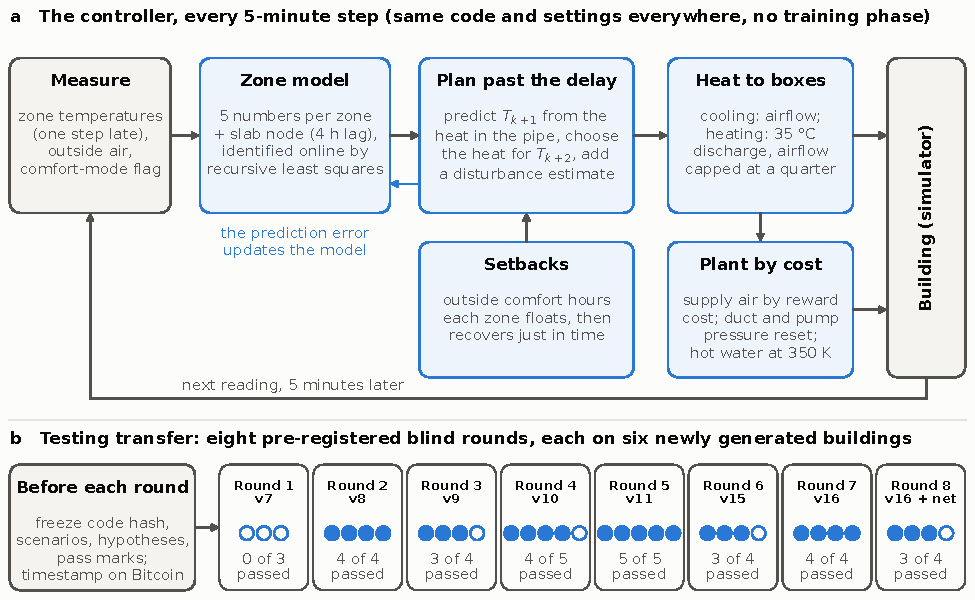
\includegraphics[width=0.81\linewidth]{../docs/fig/fig_overview.pdf}
\caption{Overview. (a) The controller runs the same code in every building and learns five numbers per zone while
the building runs. (b) Each major version (in round 8, a candidate that was not adopted) was tested in a blind round
of its own, on buildings generated from new seeds; filled circles are pre-registered hypotheses that passed, open circles hypotheses that failed.}
\label{fig:overview}
\end{figure}
% HVAC share, "as inefficiently as decades ago" and "lack of policy transfer": abstract of the contest paper
% (arXiv:2610.18511, read 30 Oct).
Heating, ventilation and air conditioning (HVAC) accounts for about 15\,\% of the world's energy use, yet most
buildings still run it about as inefficiently as they did decades ago \cite{goldfeder2026smart}. The organisers of the
Smart Buildings Challenge name the main obstacle: controllers, learned or hand-built, do not transfer. They work in the
building they were made for, and not in the next one. The challenge \cite{goldfeder2026competition} makes transfer the
task: one policy is scored on six buildings and five weather stations it has never seen, all generated by the simulator
of the Smart Buildings Control Suite \cite{goldfeder2024smart}.

We asked a simple question: does transfer need training at all? Instead of fitting a policy to the training buildings,
we first measured how the simulated building responds to heat. Then we wrote a controller whose only building-specific
part is learned online: a five-number thermal model for every zone, updated at every step. Its plans look past a
one-step delay that we found in the temperature reading (Figure~\ref{fig:overview}a). No policy is trained in advance
and nothing is tuned per building. The structure, the starting values and the global settings were fixed during
development on the shipped scenarios.

A public leaderboard shows one number, and it invites tuning to that number
\cite{blum2015ladder}. So we tested transfer the way the competition does, but again and again. Each major version met
six buildings from new generator seeds, a test we call a blind round. We pre-registered each round: before its first
run, we wrote down the hypotheses and their pass marks and sent the plan's hash for a Bitcoin timestamp. We
report every hypothesis as passed or failed (Figure~\ref{fig:overview}b). The first round failed and taught us the most.

\textbf{Contributions.}
\begin{contriblist}
\item A probe of the simulator: heat shows up in the measured temperature one step late, and the floor slab trails the
room air by about four hours (Section~\ref{sec:sim}).
\item A training-free controller that learns five numbers per zone online and plans past the delay, in about 1\,ms per
step (Sections~\ref{sec:model}--\ref{sec:schedule}).
\item Evidence of transfer: eight pre-registered blind rounds on 78 new scenarios, including a failed round and its
fix. Since the fix, the controller has beaten the strongest official baseline in all 122 scenarios outside its
development set. Ablations on blind and hidden buildings show that online learning, the slab node and the delay
handling carry the transfer (Sections~\ref{sec:protocol} and~\ref{sec:results}).
\item Two findings about the benchmark: empty US federal holidays under a comfort schedule, and full-size buildings
that reproduce much of our public-training gap (Section~\ref{sec:bench}). Last, what our results suggest for building
foundation models (Section~\ref{sec:concl}).
\end{contriblist}

\section{Related works}
The challenge's simulator, the Smart Buildings Control Suite \cite{goldfeder2024smart}, was built to calibrate against
real buildings for offline learning \cite{goldfeder2023lightweight}. SAC and DDPG agents trained in it on one building
beat its baseline policy and generalised to unseen seasons \cite{goldfeder2025rl}. Reviews of reinforcement learning
for building control report long, data-hungry training and weak transfer to new buildings \cite{wang2020rl}, which
recent benchmarks target \cite{taboga2026b2b}.
% Pinto et al.: 77 studies, deep learning in more than half (abstract, read 31 Oct); Xu et al.: shared front-end
% network, back-end trained per building (arXiv:2008.03625 abstract, read 31 Oct).
Transfer learning re-uses what was learned in source buildings; a review of 77 studies found deep learning in more
than half \cite{pinto2022transfer}. For HVAC control, one design shares a front-end network across buildings and
trains a back-end network for each \cite{xu2020onefor}. Another pre-trains a thermal model on 450 houses and fine-tunes
it on each new one \cite{raisch2025gentl}.
% Jeen et al.: arXiv:2206.14191v3 and AAAI page (read 10 Nov; abstract read again 11 Nov): no pre-training,
% commissioning period, ensemble of probabilistic networks, "outperforms an existing RBC once, and popular RL baselines
% in all cases".
Zero-shot reinforcement learning also deploys with no pre-training: after a short commissioning period it fits a
deep-network ensemble online and plans over it. It beat a rule-based controller in one of three simulated
buildings \cite{jeen2023zeroshot}. We transfer only the controller's structure and learn a handful of physical numbers
per zone online, with no training run in any building and no exploration phase. Model
predictive control (MPC) plans over a model of the building \cite{oldewurtel2012mpc,drgona2020mpc}.
% Zeng and Barooah: arXiv:2102.03856 (model updated every week, single zone, year-long simulation); Lian et al.:
% arXiv:2106.05740 abstract (20-day test, single-zone conference building). Read 10 Nov.
Adaptive versions have re-identified the model weekly in a simulated single zone \cite{zeng2021adaptive} and run for 20
days in a real one \cite{lian2023adaptive}. Grey-box models
with a slow thermal-mass node are a standard choice \cite{bacher2011greybox}, and our slab node is the simplest such
model. We identify it by recursive least squares with forgetting \cite{ljung1999system}. Together with planning past a
dead time, this is self-tuning predictive control \cite{clarke1987gpc} in a per-zone physical form. Our fix for limit
cycles is an integrating disturbance estimate, the standard route to offset-free MPC
\cite{muske2002disturbance,pannocchia2003disturbance}. Pre-registration separates generating hypotheses from testing
them \cite{nosek2018preregistration}.

\section{Methods}\label{sec:method}
% Code: policies/zonal.py (frozen code of every round: frozen/README.md); final parameters submission/V15_PARAMS.json
% (V14_PARAMS.json plus empty_day 1, empty_h 1.0).
The controller runs the same code and settings in every building. At start-up it reads the building's metadata
(zones, air handlers, setpoint ranges) and nothing else. Algorithm~\ref{alg:step} in
Appendix~\ref{app:settings} lists one control step.

\subsection{The simulator, as the controller sees it}\label{sec:sim}
% Reward: smart_control/reward/setpoint_energy_carbon_regret.py and the scenario config.gin files. Electricity vs gas:
% electricity_energy_cost.py (16-20 cents/kWh; 88-105 g CO2/kWh), natural_gas_energy_cost.py (2.3-3.1 cents/kWh;
% 181 g/kWh); marginal reward per kWh at mean prices, cost and carbon each normalised by the plant maxima: 2.1.
\textbf{Reward.} Each five-minute step is scored as $r=-(0.6\,p+0.2\,E+0.2\,C)$. The competition's score is the
mean of $-r$ over all steps; we call it the loss, and its part $0.6\,p$ the comfort term. The discomfort $p$ counts
only occupied zones; summed over a run, we call it the comfort regret. Each occupant's
discomfort grows with the distance from the comfort band (294--297\,K), linearly up to 5\,K and quadratically beyond.
The sum is divided by the number of occupants, so one person alone in a cold zone weighs as much as a full floor.
Energy cost $E$ and carbon $C$ count at every step, normalised by the plant's maximum
rates (80\,kW of electricity and 205\,kW of gas per air handler).

% Plant limits: simulator/air_handler.py (max_recirculation 0.7; the handler only cools), simulator/vav.py
% (max_discharge_air_temperature 308.15 K), config.gin (damper floor, static-pressure floor), boiler.py.
\textbf{Plant limits.} The air handlers can only cool, and at least 30\,\% of their supply air is outside air. All
heat comes from a boiler, through a reheat coil in each zone's variable-air-volume (VAV) box, whose discharge air is
capped at 35\,$^\circ$C.
Dampers cannot close below 10\,\%, and the duct static pressure cannot fall below 200\,Pa. These limits put a floor
under the energy any controller can reach (Appendix~\ref{app:loss}).

% Probe: sb/probe.py, sb/fit_probe.py (16 Oct); docs/TUNING_LOG.md (probe split by sign).
\textbf{Probe.} Before writing any controller, we drove building 1 (39 zones, Atlanta weather) with random heat for
600 steps and fitted models of each zone's temperature change (Appendix~\ref{app:probe}). A model in which heat
acts within the same step explains little ($R^2=0.44$). Letting the heat act one step later raises it to 0.63, and
adding relaxation of the room air towards its surroundings raises it to 0.87. Heating and cooling share the same
one-step delay. Another participant later traced it to the zone-temperature reading, which reports the state of the
previous step, and the organisers ruled that it stays for the competition (forum, October 2026). A second, slower
effect appeared in long cold runs: the floor slab follows the room air about four hours behind, which a first-order
model cannot represent.

\subsection{A thermal model for each zone, learned online}\label{sec:model}
% Model check: docs/TUNING_LOG.md (v11, offline 6-h RMSE in fairbanks_1: 7.10 K for v10's model, 0.94 K for Eq. 1);
% m2_forget 0.998 in frozen/zonal_v14f.py.
Each zone $z$ has the model
\begin{equation}\label{eq:m2}
\begin{aligned}
T_{z,k+1}-T_{z,k} &= -\lambda_z (T_{z,k} - T^{m}_{z,k}) + g_z\, q_{z,k-1} + c_z + b_z (T^{\mathrm{oa}}_k - T_{z,k})
  + c^{\mathrm{cm}}_z\, \mathbf{1}_{\mathrm{comfort}},\\
T^{m}_{z,k+1} &= T^{m}_{z,k} + (T_{z,k} - T^{m}_{z,k})/48,
\end{aligned}
\end{equation}
where $T_{z,k}$ is the measured temperature of zone $z$ at step $k$, $q_{z,k-1}$ the heat its box delivered one step earlier (the
delay), $T^{m}$ a slow node for the slab that follows the room air with a lag of 48 steps (four hours),
$T^{\mathrm{oa}}$ the outside temperature and $\mathbf{1}_{\mathrm{comfort}}$ the building's comfort-mode flag, which
switches internal gains on. The five numbers per zone ($\lambda_z, g_z, c_z, b_z, c^{\mathrm{cm}}_z$) start from the
medians of offline fits on four training traces. They are then updated at every step by recursive least squares with
a forgetting factor of 0.998. Every parameter has bounds, the prediction error is clipped and the covariance is
bounded (Table~\ref{tab:numbers}), because an unbounded version diverged during development. The slab node is
essential. In Fairbanks, the first-order model of our earlier versions (no slab, no outside-air term) predicted six
hours ahead with an error of 7.1\,K, against 0.9\,K for Eq.~\ref{eq:m2}, and removing the slab node doubled v11's
training loss (Appendix~\ref{app:abl}).

\subsection{Planning past the delay}\label{sec:plan}
The heat commanded now acts on the next step, and the temperature it produces is read one step after that. At step
$k$ the controller therefore predicts $T_{k+1}$ from the heat already in the pipe (commanded one step earlier), and
then where the zone would be at $k+2$ with no further heat. It chooses $q_k$ to move $T_{k+2}$ a damped fraction of
the way to a target just inside the comfort band. This is dead-time compensation, the idea of the Smith predictor
\cite{smith1957deadtime}. A per-zone disturbance estimate, a smoothed average of the model's recent errors, is added
to every prediction. This is the integrating disturbance of offset-free MPC
\cite{muske2002disturbance,pannocchia2003disturbance}: without it, a zone whose model sits at a parameter bound never
reaches its target. A safety net gives full effort to a zone far outside its band. On the cooling side it fires
only if the heat already in the pipe will not bring the zone back, and never in a zone that was asked for heat in the
last two steps. Section~\ref{sec:cycle} shows why these parts are needed.

\subsection{From heat to actuators}
For cooling, the box airflow follows from the heat to remove and the supply-air temperature. For heating, the box
discharges at the 35\,$^\circ$C cap and its airflow is limited to a quarter of the box maximum, as in the dual-maximum
logic of Guideline~36 \cite{ashrae2021g36}. Supply air is at least 30\,\% outside air that the reheat
coil must also warm, so more air at a lower discharge temperature costs more gas for the same heat. Zones already
below their band get a higher cap. Zones that need nothing
get the damper's minimum position, and if even that airflow would over-cool them, just enough reheat.

\subsection{Air-handler and plant setpoints by estimated cost}
For each air handler, the controller tries a few supply-air temperatures and picks the one with the lowest estimated
cost in reward units: fan power, chiller electricity, the reheat that colder air will need, and a penalty for cooling
demand it cannot meet. As in Guideline~36
\cite{ashrae2021g36}, the duct static pressure is reset from the most open damper, and the hot-water pump pressure to the
lowest value at which every open reheat coil still reaches its planned discharge temperature. The hot-water supply temperature is held at 350\,K, so our scores do
not depend on an accounting issue reported in the simulator's tank model (Appendix~\ref{app:tank}).

\subsection{Schedule, setbacks and empty days}\label{sec:schedule}
The comfort period is read from the metadata and re-aligned whenever the building's comfort flag switches at a
different hour. Outside it, the band widens to the building's wider eco band, and two setbacks, which let zones drift
while nobody is expected, save most of the night energy. In the
heating season (24-hour mean outside temperature below 18.3\,$^\circ$C), each zone may float down towards a low floor,
but never below the temperature from which its own model can still bring it back in time:
\begin{equation}\label{eq:glide}
T^{\mathrm{floor}}_z(k) = \max\!\Big(T_{\mathrm{eco}}-\Delta,\; \min\big(T^{*},\; T^{*} - \alpha\, \hat r_z(k)\,\max(N_k-2,0)\big)\Big),
\end{equation}
where $T^{*}$ is the lower edge of the comfort band plus margins (0.38\,K), $\hat r_z$ the zone's net heating rate at the recovery
airflow cap predicted by Eq.~\ref{eq:m2}, $N_k$ the number of steps left until the comfort period, $\alpha=0.66$ a
safety factor and $\Delta=16$\,K the deepest float. Each zone thus starts its own recovery at the last safe moment
(Figure~\ref{fig:glide} in Appendix~\ref{app:figs}). Cooling mirrors this: at night a zone may float up only as far as
its predicted cooling rate can undo in time. Finally, the empty-day rule: a work day on which nobody has come in an
hour after the comfort period starts is run as unoccupied (Section~\ref{sec:holiday}).

\subsection{How we tested: blind rounds}\label{sec:protocol}
% docs/PREREGISTRATION*.md (rounds 1-6), docs/DEVIATIONS.md, sb/make_heldout.py.
% Baseline: starter kit smart_buildings/baselines/pid_plus.py, class PIDWaterResetPolicy. Drafts v3-v6:
% docs/TUNING_LOG.md (first lines).
\textbf{Baseline and versions.} We compare against pid\_water, the strongest official baseline: PID zone
control with proportional reheat and a hot-water temperature reset on demand. Our frozen versions (code and
settings fixed before the test) are v7 to v16; lower numbers were drafts.

\textbf{Development.} Decisions used development scenarios only: the 30 shipped training scenarios (after round 1 at
full length) and buildings we generated for development, never a blind round's buildings before its run.

\textbf{Blind rounds.} Each round used six new buildings from the competition's generator, with seeds that no run had
used, scaled to the size range of the shipped buildings. They ran in twelve 30-day weather windows, including
Minneapolis, a station absent from training; some windows overlap development weather (Appendix~\ref{app:wx}). Before
any run, we froze the controller's code (by its
hash), the scenarios, the hypotheses and their numeric pass marks, and sent the plan's hash to OpenTimestamps
\cite{todd2016opentimestamps}, which commits it to a Bitcoin block (Appendix~\ref{app:stamps}). Rounds 6--8 differ: six buildings at
full size (the generator's default, larger than the shipped buildings; Section~\ref{sec:big}), with one ten-day window
each. Every hypothesis is reported as passed or failed (Table~\ref{tab:hyp}).
Deviations are logged in the repository; none changed a number.

\section{Results}\label{sec:results}
% Table 1: docs/RESULTS_EXTERNAL.md (public scores), RESULTS_HELDOUT.md, RESULTS_ROUND2..6.md (round 6: 0.012247
% against 0.012583), TUNING_LOG.md (v12 = v11 + boost_k 0.25; v13 = v12 + glide_floor -16, f_heat_rec 0.35;
% v14 = v13 + offset_free 3); v15: docs/HOLIDAY.md (full-length check, results/holiday/ed1_full).
Table~\ref{tab:main} lists every frozen version, what it added and how it did. Figure~\ref{fig:overview}b shows which pre-registered hypotheses passed (paired
statistics in Appendix~\ref{app:stats}): round 1 failed, rounds 2, 5 and 7 passed every hypothesis, and rounds 3, 4, 6
and 8 each failed one. We take the results as answers to four questions.
\begin{table}[!htb]\centering
\caption{Every frozen version, what it added, and its mean loss per step (lower is better). Training: the 30 shipped
scenarios at full length. Blind round: 12 new scenarios on six new buildings (rounds 6 and 7: six full-size
buildings, ten days each), with the previous version and pid\_water, the strongest official baseline (run after rounds
6 and 7). Public: Kaggle public leaderboard. All policies: Tables~\ref{tab:grid} and~\ref{tab:grid68}.}\label{tab:main}
\small
\setlength{\tabcolsep}{3.5pt}
\begin{tabular}{l>{\raggedright\arraybackslash}p{3.4cm}cccccc}\toprule
 & & & \multicolumn{4}{c}{Blind round} & \\\cmidrule(lr){4-7}
Version & What it added & Training & No. & Loss & Previous & pid\_water & Public\\\midrule
v7 & first frozen controller & 0.03185 & 1 & 0.03298 & -- & 0.03572 & --\\
v8 & fixes for limit cycles & 0.01252 & 2 & 0.01016 & 0.03048 & 0.04378 & 0.01687\\
v9 & heating setback (Eq.~\ref{eq:glide}) & 0.01199 & 3 & 0.02063 & 0.02223 & 0.07424 & 0.01623\\
v10 & CMA-ES re-tune & 0.01092 & 4 & 0.02043 & 0.02177 & 0.06922 & 0.01543\\
v11 & slab node, pump reset, cooling setback & 0.00744 & 5 & 0.00827 & 0.01145 & 0.05519 & 0.01071\\
v12 & earlier heating boost & 0.00739 & & & & & 0.01058\\
v13 & deeper night float, faster recovery & 0.00735 & & & & & 0.01051\\
v14 & droop fix (App.~\ref{app:stress}) & 0.00733 & & & & & 0.01048\\
v15 & holiday rule & 0.00719 & 6 & 0.01225 & 0.01258 & 0.05946 & 0.01035\\
v16 & no cooling right after heating, smaller margin & 0.00716 & 7 & 0.01630 & 0.01765 & 0.10017 & 0.01031\\\midrule
pid\_water & official baseline & 0.05414 & & & & & 0.06404\\\bottomrule
\end{tabular}
\end{table}
% sb/fig_transfer.py (31 Oct): counts and ratios printed by the script. Unseen sets: results/heldout..heldout5 (rounds
% 1-5, each round's frozen version and pid_water), results/stress (v13), results/bigbld and results/bigdev (v14),
% results/round6h (v15), results/round7 and results/round8 (v16), with pid_water run there after the rounds (docs/BASELINE_R67.md).
% Cold start: docs/COLD_START.md (rules written 8 Nov 23:36 and sent for a timestamp before any run; read 9 Nov 00:03);
% sb/run_coldstart.py --read, policies/zonal_v16_coldstart.py.
% First work day: the first weekday that is not a US federal holiday; 60 windows start on a Sunday, 20 on a Saturday
% and 8 at 06:00 on a Friday (round 3 and 4, 1 December), where the first day's ratio is 0.17-0.37 against 0.13-0.42.
\begin{figure}[t]\centering
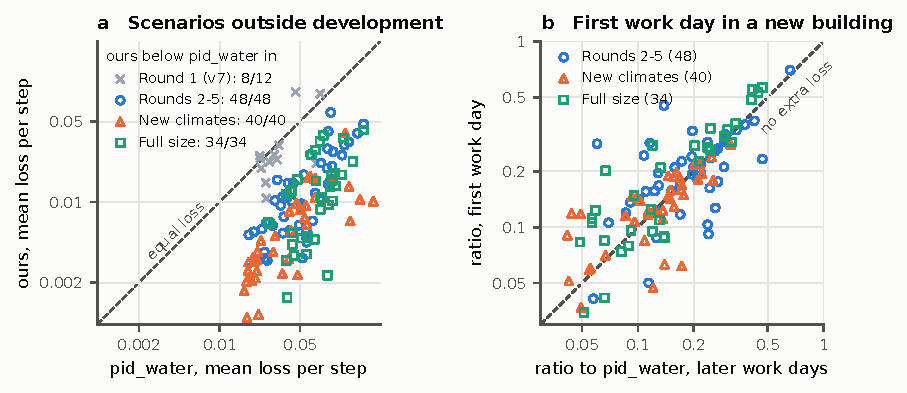
\includegraphics[width=0.82\linewidth]{../docs/fig/fig_transfer.pdf}
\caption{Transfer. (a) Every scenario outside development: our frozen version's mean loss per step against pid\_water's
(log scales; below the dashed line ours is lower). (b) Rounds 2--5, new climates and full-size buildings: loss ratio to pid\_water on the first work day against the later work
days; points on the line mean no extra loss on the first work day.}
\label{fig:transfer}
\end{figure}
\subsection{Does it transfer?}\label{sec:transfer}\label{sec:kaggle}\label{sec:stress}
From v8 on, yes (Figure~\ref{fig:transfer}a). v7 was below pid\_water in
8 of 12 scenarios of round 1. From v8 on, the frozen version was below it in every scenario: 48 of 48 in rounds 2--5,
40 of 40 on the training buildings in ten climates absent from training (Appendix~\ref{app:stress}) and 34 of 34 on 26
full-size buildings (18 new ones in rounds 6--8, eight of rounds 1 and 5 run unscaled in Section~\ref{sec:big}). Its
loss was typically four to seven times lower (median ratios 0.23, 0.15 and 0.15).
% audit/split.py (11 Nov 2026; descriptive, from the result files): over the 122 scenarios, each counted once, our
% comfort term is 0.00135 against pid_water's 0.04248 (3.2 %), our energy and carbon part 0.01086 against 0.01863
% (58.3 %); the comfort term is 84.1 % of the gap; our energy and carbon part is lower in 94 of 122.
The gap is mostly comfort (84\,\% of it): over the 122 scenarios our comfort term is 3\,\% of pid\_water's and our
energy and carbon part 58\,\% (Table~\ref{tab:split}).
On the first work day the loss ratio to pid\_water (medians 0.20, 0.13 and 0.14) is close to that of the later work
days (0.20, 0.14, 0.13; Figure~\ref{fig:transfer}b), but most windows start on a weekend. For a true cold
start we restarted v16 from nothing at 06:00 on the first work day of the twelve full-size windows of rounds 6 and 7.
That day's loss is 1.20 times v16's (95\,\% interval 1.09--1.34), still below pid\_water in all twelve, and the next
work day's is 1.01 times (Appendix~\ref{app:abl}).

% docs/RESULTS_EXTERNAL.md; docs/STRESS_TEST.md (details in Appendix~\ref{app:stress}); docs/FIXSIM.md (rule written
% before any run; read 4 Nov 16:48 and 17:32).
On the public leaderboard (about a third of the hidden test set) v16 scores 0.01031. We submitted every frozen version from v8 on; none had a parameter chosen by its public score. These scores do
not rest on the simulator's reported energy issues: with both proposed fixes (Appendix~\ref{app:tank}), v16's loss
rises by 2.1\,\% in six cold and 0.1\,\% in six hot full-size windows, and it stays below pid\_water in all twelve. Our
public scores have been 1.35--1.44 times our training scores, against 1.18 for pid\_water submitted unchanged
(Appendix~\ref{app:lb}). New climates are not the reason (Appendix~\ref{app:stress}); building size may be
(Section~\ref{sec:big}).

% docs/TRAINED_BASELINE.md (plan and reading rules timestamped before training); sb/run_trained.py --read
% (results/rl_test/summary.json).
We also trained a policy, since the starter kit ships none: two small networks, shared across zones and air
handlers, correct pid\_water's commands. PPO trained them on five training buildings for 38
hours (3.3 million simulator steps; Appendix~\ref{app:trained}). On the twelve buildings of Table~\ref{tab:what} its
loss is 0.89 times pid\_water's (below it in 11 of 12) and 5.0 times v16's (v16 lower in 12 of 12).
Its gain is energy: it keeps 95\,\% of pid\_water's comfort term, which v16 all but removes.
% Kaggle Submissions page, read 11 Nov 2026 20:52 UTC: trained residual 0.03911 (pid_water 0.06404, v16 0.01031).
On the public leaderboard it scored 0.03911, 0.61 times pid\_water's score and 3.8 times v16's.

\subsection{What carries the transfer?}\label{sec:what}
% docs/TRANSFER_ABLATION2.md (rules written 8 Nov 19:05, before any run; hash c7903b7ae0fff60e sent for a timestamp;
% results read 8 Nov 23:37; sb/run_transfer_abl2.py --read).
% docs/TRANSFER_ABLATION.md (variants and reading rules written and timestamped 31 Oct 07:04, block 973,939, before
% any run; results read 31 Oct 09:06 and 09:24); sb/run_transfer_abl.py --read, --days; results/transfer_abl;
% policies/zonal_v16_offsetonly.py (known-answer check passed). Learned gains: sb/params_read.py (size-gate traces of
% v15, day 3; shipped zones median 0.275; six full-size buildings: medians 0.142-0.295, max/min within a building
% 2.0-3.6; computed 31 Oct, written 12:05 by `date`; docs/TRANSFER_ABLATION.md).
\begin{table}[t]\centering
\caption{What carries the transfer: v16 with one part changed, on the twelve full-size buildings of rounds 6 and 7
(ten days each; post hoc, with the variants and reading rules timestamped before the runs). Loss: mean loss relative
to v16's, with a 95\,\% bootstrap interval over buildings. Worse in: buildings where the variant's loss is higher.
Comfort: mean comfort term per step. Public: Kaggle public
score, on hidden buildings, relative to v16's 0.01031 (one score each).}\label{tab:what}
\small
\begin{tabular}{lcccc}\toprule
Variant of v16 & Loss / v16 & Worse in & Comfort & Public\\\midrule
v16 & 1 & -- & 0.00048 & 1\\
no online learning (priors only) & 2.68 (2.27--3.23) & 12 of 12 & 0.02582 & 1.50\\
only the disturbance estimate learned & 1.16 (1.06--1.28) & 11 of 12 & 0.00313 & 1.00\\
priors halved, learning on & 1.02 (1.01--1.04) & 12 of 12 & 0.00065 & 1.01\\
priors doubled, learning on & 1.01 (0.97--1.06) & 7 of 12 & 0.00091 & 1.00\\
no delay compensation in planning & 1.02 (1.005--1.04) & 12 of 12 & 0.00067 & 1.14\\\bottomrule
\end{tabular}
\end{table}
After round 7 we changed one part of v16 at a time (Table~\ref{tab:what}; Figure~\ref{fig:what} in
Appendix~\ref{app:abl}). Online learning carries the transfer. With every zone's five numbers frozen at their starting values and no disturbance estimate, the
loss is 2.7 times v16's and higher in all twelve buildings; the whole rise is discomfort on work days. Learning only the
disturbance estimate closes most of that gap, but the loss stays 16\,\% above v16's. The starting values matter little:
halved, they cost 2\,\% over ten days; doubled, 1\,\%. In full-size buildings the learned gains differ by building
(medians 0.14--0.30) and, within a building, by a factor of 2--3.6 between zones: what transfers is the procedure that
finds each zone's numbers, not the numbers themselves. Planning past the delay alone is worth less than its 5\,\% mark: without it
the loss rises by 2\,\% (worse in all twelve), because two other parts respond to the same lag. With all three off (planning, the delay-aware safety net and the rule against
cooling right after heating, Section~\ref{sec:r7}), the loss is 14\,\% higher (interval 1.03--1.30). It is worse in
all twelve, but by 19--119\,\% in only four of them (Table~\ref{tab:what2} in Appendix~\ref{app:abl}). The slab node is
worth 16\,\% (interval 1.09--1.27). Its fixed four-hour lag need not be exact: two or eight hours change the loss by
$-0.8$ and $+1.8$\,\%.

% docs/PUBLIC_ABLATION.md (reading rules written and timestamped before any build; block 975,079; scores read 9 Nov 07:32 UTC);
% docs/PUBLIC_ABLATION2.md (rules timestamped before any build; block 975,121; scores read 10 Nov 07:31 UTC).
The same variants went to the public leaderboard, which scores buildings we have never seen (last columns of
Tables~\ref{tab:what} and~\ref{tab:what2}; rules timestamped before submission). Learning again carries the transfer:
without it the score is 1.50 times v16's, and halved or doubled starting values give 1.01 and 1.00 times. Learning only
the disturbance estimate matches v16 (1.00), so on those windows the five numbers add nothing measurable beyond that
estimate. The probe's two facts weigh more there: without planning past the delay the score is 1.14 times v16's,
without any delay handling 1.23 times and without the slab node 1.78 times, while a two- or eight-hour lag changes
it by at most 1.5\,\%.

% sb/figures.py cycle (zone dumps results/zones_atl2_d16*.npz); docs/TUNING_LOG.md (round-1 diagnosis).
\begin{figure}[t]\centering
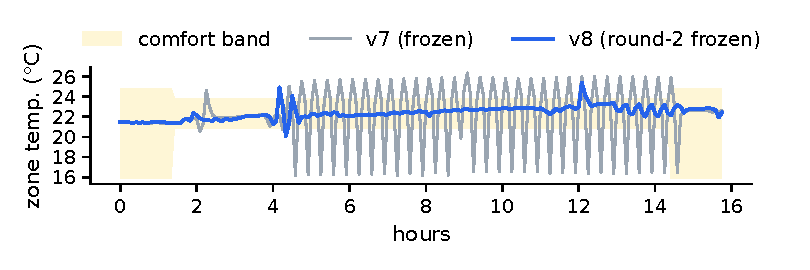
\includegraphics[width=0.72\linewidth]{../docs/fig/fig_cycle.pdf}
\caption{The failure of round 1: one zone on one warm day (training scenario: building 1, Atlanta, day 16). v7 (grey)
cycles every four steps; v8 (blue), with the delay-aware safety net and the disturbance estimate, holds the band.}
\label{fig:cycle}
\end{figure}
\subsection{What did the failures teach?}\label{sec:cycle}\label{sec:r2}\label{sec:r7}
% docs/RESULTS_HELDOUT.md; docs/TUNING_LOG.md (round-1 diagnosis); fig_cycle.png; docs/RESULTS_ROUND2.md;
% docs/RESULTS_POSTHOC_R1.md.
\textbf{A relay with dead time (rounds 1 and 2).} v7, frozen for round 1, was only 7.7\,\% below pid\_water, against a
pass mark of 30\,\%, and all three hypotheses failed. The cause showed only in runs longer than our ten-day development
runs: on day 16 of a warm training scenario, 21 of 39 zones swung between 16 and 26\,$^\circ$C in a four-step limit
cycle (Figure~\ref{fig:cycle}). Two mechanisms fed it. First, the safety net gave full effort to
zones that the heat already in the pipe was about to bring back. A full-effort rule acting on a reading that lags its
own effect is a relay with dead time, which oscillates \cite{astrom1984relay}. Second, zone models stuck at a parameter
bound kept missing their target. v8 fixes both, with the delay-aware safety net and the disturbance estimate of
Section~\ref{sec:plan}. In round 2 all four hypotheses passed: v8 was 66.7\,\% below v7 and 76.8\,\% below pid\_water,
and better than v7 in all 12 scenarios.

% docs/HEATLESS.md (margin screen: rule 30 Oct 18:17, result 20:47); docs/CHATTER.md (trace of building_train_8
% atlanta_1, zone 20; option; screen rule 30 Oct 23:40, result 31 Oct 03:21); docs/PREREGISTRATION_7.md (written
% 30 Oct 23:43, stamped 31 Oct 03:21:35, before generation); docs/RESULTS_ROUND7.md (read 31 Oct 04:21).
\textbf{The same relay in small rooms (round 7).} A smaller heating margin (aiming 0.30 instead of 0.40\,K inside the
band) lowered the loss by 1.6\,\% in six cold full-size development windows (Appendix~\ref{app:sens}). But it tipped a
fast zone of one training window into the same relay, now between the two safety nets: one step of full heat lifted it
by 8\,K, the late reading fired full cooling, and the cycle repeated for ten hours. v16 adds one
rule, cool-hold: a zone asked for heat in one of the last two steps is not cooled. In round 7 (six new full-size
buildings, cold ten-day windows) v16 was 7.6\,\% below v15 and better in all six, with half the comfort regret. The
rule alone gave 7.55 of the 7.64\,\%. Most of the gain came from New York ($-10.6$\,\%) and Chicago ($-21.4$\,\%), and
there from the smallest rooms (20--27\,m$^2$). Under v15 these switched between full heating and full cooling
15--68 times every work day and held 90--96\,\% of the occupied discomfort (Figure~\ref{fig:r7}).

% docs/RESULTS_ROUND3.md, RESULTS_ROUND4.md, RESULTS_ROUND5.md; fig_glide.png, fig_round5.png; TUNING_LOG.md (v12-v14
% rules written before their runs); docs/RESULTS_ROUND8.md.
\textbf{Smaller lessons.} v9's heating setback (Eq.~\ref{eq:glide}) was 9.1\,\% below v8 in round 3's cold scenarios
but failed its comfort hypothesis ($+7$\,\% comfort regret). v10, a re-tune of 14 settings by CMA-ES
\cite{hansen2001cma} on six training scenarios, gained 19.7\,\% in round 4's warm scenarios and lost 0.2\,\% in the cold
ones: the search did not carry over. v11 (slab node, pump and cooling resets) passed all five hypotheses of round 5,
27.8\,\% below v10 (Figure~\ref{fig:r5}, Table~\ref{tab:abl11}). In round 8 a heating net that also waits for the heat
in the pipe gained only 0.12\,\% (mark 0.3\,\%), so v16 stays (Appendix~\ref{app:r8}).

\subsection{What did we learn about the benchmark?}\label{sec:bench}\label{sec:holiday}\label{sec:big}
% docs/HOLIDAY.md (simulator code read 30 Oct; bound; screen; full-length check of 70 windows, read 07:50; false
% alarms: fewest occupants in a building on disk 36, (35/36)^(12*36) = 5e-6); docs/PREREGISTRATION_6.md (fixed and
% stamped 30 Oct 02:18, before generation); docs/RESULTS_ROUND6.md; docs/DEVIATIONS.md (deviation 6);
% sb/run_holiday.py, sb/make_round6h.py, sb/run_round6h.py; simulator randomized_arrival_departure_occupancy.py,
% setpoint_schedule.py. Public score: docs/RESULTS_EXTERNAL.md (prediction written 30 Oct 07:50, score read 15:20).
\textbf{Empty holidays (round 6).} On US federal holidays the simulator's occupancy model keeps everybody at home, but
the setpoint schedule stays in comfort mode, and the comfort term is zero when nobody is in. v14 held the band anyway.
The controller does not see the date, but it does see the occupant count. On a normal work day the
chance that nobody has come in by 07:00 is below $10^{-5}$ in every building we ran. v15 therefore adds the empty-day rule of Section~\ref{sec:schedule}, a whole-building
version of the occupied-standby mode of Guideline~36 \cite{ashrae2021g36}. In round 6 (six new
full-size buildings, ten days around six holidays) v15 was 2.67\,\% below v14 and better in all six; its comfort
hypothesis counts as failed (Table~\ref{tab:hyp}). On the public leaderboard v15 scored 1.2\,\% below v14, within the 1--2\,\% we had
predicted.

% docs/BIG_BUILDINGS.md (rule, six pairs, diagnosis 1), docs/BIGDEV.md (diagnosis 2, rules of the earlier, failed
% "v15" candidates of 25-27 Oct; the final v15 is the holiday rule), sb/make_bigbld.py, sb/bigbld_eval.py,
% sb/bigbld_dump.py, sb/bigbld_dump_read.py; results/bigbld, results/bigbld_diag. Deep cold: docs/BIG_BUILDINGS.md
% ("Does size raise heating in deep cold?", rule 29 Oct 22:56; result 30 Oct); sb/run_coldsize.py.
\textbf{Full-size buildings.} By default the competition's generator draws buildings larger than the six shipped
ones (footprints of 400--700 by 300--500 grid units). The hidden buildings come from it at a size the starter kit
does not state, and our rounds 1--5 had scaled every building down to the shipped size. We fixed a rule before the
runs: size explains the gap between our public and training scores if v14's loss ratio to pid\_water at full size is
at least 0.160 and 1.15 times that at the shipped size. Both hold: it is 1.43 times, in three round-5 buildings run
unscaled and again in five round-1 buildings (16 pairs, 95\,\% interval 1.02--2.02; Table~\ref{tab:size}). In the replication the
rise sits in hot weather (0.141 to 0.378): a larger floor's cooling falls on the same air handlers, at the plant's
limits. Every team carries this weight if the hidden buildings are full size. In cold weather the ratio falls (0.193
to 0.135), and a deep-cold test missed its mark (Appendix~\ref{app:monday}).

\section{Conclusion}\label{sec:concl}
% Sections 3-4, no new numbers.
Probing the simulator gave the controller its shape: a five-number model per zone and plans that look past a one-step sensor lag. Learning
these numbers online is what carries it to a new building. Without learning, the same controller loses 2.7 times as
much (1.5 times on the public leaderboard). Since round 1's fix it has beaten the strongest official baseline in all
122 scenarios outside development.

% The open question: contest paper, Section 1.5 "Scientific challenge" (arXiv:2610.18511v1, read 10 Nov).
\textbf{What this suggests for building foundation models} (our reading). The organisers leave open whether
domain-specific models or generic foundation models will generalise best \cite{goldfeder2026smart}. Ours is
domain-specific, and three things in it bear on that question. First, what transfers here is small and
local: five physical numbers and an offset per zone, found online within about a day. A learned policy conditioned on
such per-zone estimates, or on a short history from which they follow, may transfer where a policy fitted to whole
buildings does not. Second, structure matters: the sensor lag and the slab. A
policy that acts at full effort on the lagged reading limit-cycles (rounds 1 and 7), and a model without a slow slab
state mispredicts cold nights (without it v11's training loss doubled and v16's public score rose 1.8 times). Third,
transfer should be measured as it is deployed: on full-size buildings, through holidays, and on buildings generated
after the plan is fixed.

\textbf{Limitations.} The one-step delay belongs to this simulator's sensor reading and the four-hour lag to its
buildings. A real building needs its own probe, and nothing here has run in one. Under sensor faults
(Appendix~\ref{app:faults}), noise costs 1\,\%, one more step of delay 50\,\% (nothing once it is set), and dead
sensors in a tenth of the rooms more than double the loss. Apart from Minneapolis, our blind rounds used weather
stations we had run in development, while the hidden test set uses five unseen ones. Size explains only part of the
extra public heating (Appendix~\ref{app:lb}), and the holiday rule fits this simulator only. The ablations of
Section~\ref{sec:what} ran on buildings already used and, on hidden buildings, give one public score per variant.
Empty zones cool to $-1.7\,^\circ$C in deep cold; a 5\,$^\circ$C frost floor costs 0.7\,\%
(Appendix~\ref{app:frost}). Our public score is far from the top of the leaderboard, and the trained comparison (one
architecture, budget and seed) says little about what training can reach.

\section*{AI assistance, code and compute}
The author used an AI assistant (Claude, Anthropic) to write the code and to draft the text, then reviewed the paper
and verified its results. Code, plans and proofs are public on GitHub (\href{https://github.com/abdullahcengil/training-free-hvac-sb26}{abdullahcengil/training-free-hvac-sb26}); the raw result files will follow. All runs
used the CPU of one laptop with 16\,GB of memory.

\bibliographystyle{plainnat}
\bibliography{refs}

\clearpage
\appendix
\raggedbottom
\section{Probe of the simulator}\label{app:probe}
Figure~\ref{fig:probe} shows the fits behind Section~\ref{sec:sim} and the response to heat by lag.
\begin{figure}[!htb]\centering
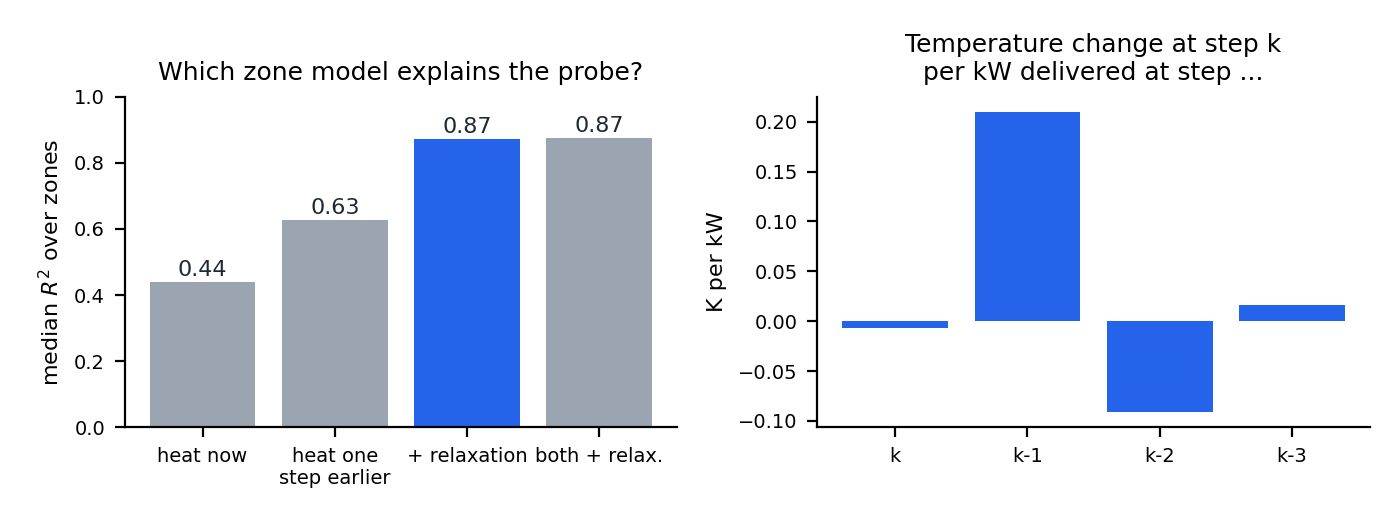
\includegraphics[width=\linewidth]{../docs/fig/fig_probe.png}
\caption{Probe of the simulator (building 1, Atlanta, 39 zones, 600 steps of random heat). Left: median $R^2$ over zones of four
per-zone models; heat at both lags (right bar) adds nothing to the one-step delay with relaxation. Right: coefficients of one regression, pooled over zones, of $T_{k+1}-T_k$ on the heat at steps $k$ to $k-3$, $T_k-295$\,K and a constant; heat acts one step late.}
\label{fig:probe}
\end{figure}

\section{All results and paired statistics}\label{app:stats}
\paragraph{Weather of the blind rounds.}\label{app:wx}
The buildings were new in every round; the weather was not always. Rounds 1 and 2 used strips that none of our runs
had used (round 2's six non-Minneapolis strips are shipped training strips not yet used in our development). Round 3's
six warm windows are shipped training strips that our development runs had used with other buildings; its cold
windows are new (Denver's overlaps a training strip by four days). Rounds 4 and 5 used new 30-day windows that overlap
training strips by up to ten days, and round 4 also reused test windows of rounds 1--3. In rounds 7 and 8 the New York
and Duluth windows from 29 January lie inside the stress test's windows from 15 January (Appendix~\ref{app:stress}),
and round 8's San Francisco window overlaps one by nine days. Counted over the 78 blind-round scenarios (from the plans'
weather lists), 45 use a window none of our earlier runs had touched, 16 overlap a strip we had used by at most ten
days per strip, and 17 repeat a window used before (6 in development, 9 as test windows of earlier rounds, 2 inside the
stress test). So the rounds test new buildings throughout, and new weather only in part.
Table~\ref{tab:grid} gives every policy in rounds 1--5, including the official baselines that ran only in rounds 1
and 2. Table~\ref{tab:grid68} gives the full-size rounds 6--8. Table~\ref{tab:split} splits the gap to pid\_water
into comfort and energy: pid\_water's loss is 70\,\% comfort term, and holding comfort is most of our advantage. Our
energy and carbon part is also lower, by 42\,\% on average, but not everywhere: at full size it is higher than
pid\_water's in 13 of 34 scenarios, and there the whole advantage is comfort. Table~\ref{tab:stats} gives the paired
comparisons behind the hypotheses, Table~\ref{tab:statsb} the same comparisons with each building counted once, and
Table~\ref{tab:hyp} all 33 hypotheses with their pass marks.
\begin{table}[!htb]\centering
\caption{All policies in rounds 1--5: mean loss per step (lower is better). Training: the 30 shipped scenarios at full length (baselines from the shipped returns). Rounds 1--5: 12 scenarios each on six new buildings, pre-registered. Bold: the version frozen for that round; v8 on round 1 was run after that round was open (post hoc).}\label{tab:grid}
\small
\begin{tabular}{lcccccc}\toprule
Policy & Training (30) & Round 1 & Round 2 & Round 3 & Round 4 & Round 5\\\midrule
bang\_bang & 0.2252 & 0.20279 & 0.22406 & -- & -- & --\\
fixed\_setpoint & 0.06592 & 0.04539 & 0.08112 & -- & -- & --\\
pid & 0.06736 & 0.04355 & 0.05520 & -- & -- & --\\
pid\_water & 0.05414 & 0.03572 & 0.04378 & 0.07424 & 0.06922 & 0.05519\\
v7 & 0.03185 & \textbf{0.03298} & 0.03048 & -- & -- & --\\
v8 & 0.01252 & 0.01011 (post hoc) & \textbf{0.01016} & 0.02223 & -- & --\\
v9 & 0.01199 & -- & -- & \textbf{0.02063} & 0.02177 & --\\
v10 & 0.01092 & -- & -- & -- & \textbf{0.02043} & 0.01145\\
v11 & 0.00744 & -- & -- & -- & -- & \textbf{0.00827}\\
v12 & 0.00739 & -- & -- & -- & -- & --\\
v13 & 0.00735 & -- & -- & -- & -- & --\\
v14 & 0.00733 & -- & -- & -- & -- & --\\
v15 & 0.00719 & -- & -- & -- & -- & --\\
v16 & 0.00716 & -- & -- & -- & -- & --\\\bottomrule
\end{tabular}
\end{table}
% docs/RESULTS_ROUND6.md, RESULTS_ROUND7.md, RESULTS_ROUND8.md, BASELINE_R67.md; round-8 means from results/round8/*.npy (first 2880 steps; 8 Nov 2026).
\begin{table}[!htb]\centering
\caption{Full-size rounds 6--8 (six new buildings each, one ten-day window each): mean loss per step (lower is better). Bold: the version or candidate under test in that round; pid\_water was run after each round.}\label{tab:grid68}
\small
\begin{tabular}{lccc}\toprule
Policy & Round 6 & Round 7 & Round 8\\\midrule
pid\_water & 0.05946 & 0.10017 & 0.07877\\
v14 & 0.01258 & -- & --\\
v15 & \textbf{0.01225} & 0.01765 & --\\
v16 & -- & \textbf{0.01630} & 0.01066\\
v16 + delay-aware heating net & -- & -- & \textbf{0.01064}\\\bottomrule
\end{tabular}
\end{table}
% audit/split.py (11 Nov 2026): descriptive, computed from the result files of every run outside development.
\begin{table}[!htb]\centering
\caption{Where the gap to pid\_water comes from: mean loss per step over the scenarios outside development, split into
the comfort term ($0.6\,p$) and the energy and carbon part (the rest). Each scenario counts once; ours is the frozen
version that ran it. Gap: share of the difference to pid\_water that is comfort. Less energy: scenarios in which our
energy and carbon part is the lower one (our comfort term is lower in all 122).}\label{tab:split}
\small
\setlength{\tabcolsep}{4pt}
\begin{tabular}{lccccccc}\toprule
 & & \multicolumn{2}{c}{Ours} & \multicolumn{2}{c}{pid\_water} & & \\\cmidrule(lr){3-4}\cmidrule(lr){5-6}
Scenarios & $n$ & comfort & energy, carbon & comfort & energy, carbon & gap & less energy\\\midrule
Rounds 2--5 (v8--v11) & 48 & 0.00303 & 0.01184 & 0.04061 & 0.02000 & 82\,\% & 35 of 48\\
New climates (v13) & 40 & 0.00022 & 0.00718 & 0.03384 & 0.01804 & 76\,\% & 38 of 40\\
Full size (v14--v16) & 34 & 0.00030 & 0.01381 & 0.05529 & 0.01738 & 94\,\% & 21 of 34\\
All & 122 & 0.00135 & 0.01086 & 0.04248 & 0.01863 & 84\,\% & 94 of 122\\\bottomrule
\end{tabular}
\end{table}
\begin{table}[t]\centering
\caption{Paired comparisons over scenarios (descriptive). Ties are identical runs. 95\,\% intervals by bootstrap over
scenarios (10{,}000 resamples); sign test $p$. $^{*}$pid\_water run after the round. From docs/RESULTS\_STATS.md
(sb/stats.py). Scenarios share buildings (two windows per building in rounds 1--5, five stations per training
building), so these tests treat dependent scenarios as independent; Table~\ref{tab:statsb} counts each building once.}\label{tab:stats}
\small
\begin{tabular}{lccccc}\toprule
Comparison & $n$ & better/same/worse & reduction & 95\,\% CI & sign $p$\\\midrule
R1: v7 vs pid\_water & 12 & 8/0/4 & 7.7\,\% & $-24.3$ to 36.9\,\% & 0.39\\
R1 (post hoc): v8 vs pid\_water & 12 & 12/0/0 & 71.7\,\% & 67.4 to 75.5\,\% & 0.0005\\
R2: v8 vs v7 & 12 & 12/0/0 & 66.7\,\% & 54.3 to 77.5\,\% & 0.0005\\
R2: v8 vs pid\_water & 12 & 12/0/0 & 76.8\,\% & 73.8 to 80.5\,\% & 0.0005\\
R3: v9 vs v8, cold & 6 & 6/0/0 & 9.1\,\% & 6.5 to 12.4\,\% & 0.031\\
R3: v9 vs v8, warm & 6 & 1/4/1 & 0.4\,\% & $-0.1$ to 1.7\,\% & 1\\
R3: v9 vs pid\_water & 12 & 12/0/0 & 72.2\,\% & 65.8 to 77.3\,\% & 0.0005\\
R4: v10 vs v9, warm & 6 & 5/0/1 & 19.7\,\% & 8.1 to 30.2\,\% & 0.22\\
R4: v10 vs v9, cold & 6 & 4/0/2 & $-0.2$\,\% & $-2.0$ to 1.5\,\% & 0.69\\
R4: v10 vs pid\_water & 12 & 12/0/0 & 70.5\,\% & 60.3 to 78.3\,\% & 0.0005\\
R5: v11 vs v10 & 12 & 12/0/0 & 27.8\,\% & 21.8 to 35.4\,\% & 0.0005\\
R5: v11 vs pid\_water & 12 & 12/0/0 & 85.0\,\% & 81.5 to 88.7\,\% & 0.0005\\
Training: v11 vs v10 & 30 & 30/0/0 & 31.9\,\% & 28.2 to 37.0\,\% & $2\times10^{-9}$\\
R6: v15 vs v14 (ten days) & 6 & 6/0/0 & 2.7\,\% & 1.6 to 4.2\,\% & 0.031\\
R6: v15 vs pid\_water$^{*}$ & 6 & 6/0/0 & 79.4\,\% & 67.5 to 87.8\,\% & 0.031\\
Training: v15 vs v14 & 30 & 23/7/0 & 1.8\,\% & 1.4 to 2.3\,\% & $2\times10^{-7}$\\
R7: v16 vs v15 (ten days) & 6 & 6/0/0 & 7.6\,\% & 0.4 to 16.7\,\% & 0.031\\
R7: v16 vs pid\_water$^{*}$ & 6 & 6/0/0 & 83.7\,\% & 77.5 to 89.7\,\% & 0.031\\
Training: v16 vs v15 & 30 & 18/11/1 & 0.4\,\% & 0.2 to 0.7\,\% & $8\times10^{-5}$\\
R8: v16 + net vs v16 (ten days) & 6 & 4/1/1 & 0.1\,\% & 0.0 to 0.8\,\% & 0.38\\
R8: v16 vs pid\_water$^{*}$ & 6 & 6/0/0 & 86.5\,\% & 79.5 to 95.1\,\% & 0.031\\\bottomrule
\end{tabular}
\end{table}
% docs/RESULTS_STATS_BUILDINGS.md (sb/stats_buildings.py, 8 Nov 2026).
\begin{table}[!htb]\centering
\caption{The comparisons of Table~\ref{tab:stats} that have several scenarios per building, with each building counted once (its scenarios averaged): six buildings per row, 95\,\% cluster bootstrap over buildings (10{,}000 resamples), sign test over buildings. With six buildings the smallest possible $p$ is 0.031.}\label{tab:statsb}
\small
\begin{tabular}{lcccc}\toprule
Comparison & better/same/worse & reduction & 95\,\% CI & sign $p$\\\midrule
R1: v7 vs pid\_water & 5/0/1 & 7.7\,\% & $-26.9$ to 39.5\,\% & 0.22\\
R1 (post hoc): v8 vs pid\_water & 6/0/0 & 71.7\,\% & 67.8 to 75.2\,\% & 0.031\\
R2: v8 vs v7 & 6/0/0 & 66.7\,\% & 50.9 to 78.8\,\% & 0.031\\
R2: v8 vs pid\_water & 6/0/0 & 76.8\,\% & 75.9 to 78.2\,\% & 0.031\\
R3: v9 vs pid\_water & 6/0/0 & 72.2\,\% & 65.5 to 78.1\,\% & 0.031\\
R4: v10 vs v9 & 6/0/0 & 6.1\,\% & 1.8 to 12.3\,\% & 0.031\\
R4: v10 vs pid\_water & 6/0/0 & 70.5\,\% & 59.2 to 78.8\,\% & 0.031\\
R5: v11 vs v10 & 6/0/0 & 27.8\,\% & 20.6 to 38.0\,\% & 0.031\\
R5: v11 vs pid\_water & 6/0/0 & 85.0\,\% & 80.5 to 89.4\,\% & 0.031\\
Training: v11 vs v10 & 6/0/0 & 31.9\,\% & 27.1 to 38.3\,\% & 0.031\\
Training: v15 vs v14 & 6/0/0 & 1.8\,\% & 1.6 to 2.1\,\% & 0.031\\
Training: v16 vs v15 & 6/0/0 & 0.4\,\% & 0.2 to 0.6\,\% & 0.031\\\bottomrule
\end{tabular}
\end{table}
% Pass marks and outcomes copied from docs/RESULTS_HELDOUT.md, RESULTS_ROUND2..8.md (8 Nov 2026).
\begin{table}[!htb]\centering
\caption{All 33 pre-registered hypotheses with their pass marks, as the frozen plans state them. Loss means the mean loss per step over the round's scenarios, ``regret'' the summed comfort regret. Round 1 tested v7; round 8 tested v16 with the delay-aware heating net against v16.}\label{tab:hyp}
\footnotesize
\begin{tabular}{clcc}\toprule
Round & Hypothesis and pass mark & Observed & Result\\\midrule
1 & v7 loss at least 30\,\% below pid\_water & 7.7\,\% & failed\\
1 & better than every baseline in at least 10 of 12 & 8 & failed\\
1 & regret at most 10\,\% of pid\_water's & 56.1\,\% & failed\\\midrule
2 & v8 loss at least 20\,\% below v7 & 66.7\,\% & passed\\
2 & better than v7 in at least 10 of 12 & 12 & passed\\
2 & loss at least 30\,\% below pid\_water & 76.8\,\% & passed\\
2 & regret at most v7's & 302 vs 2363 & passed\\\midrule
3 & v9 at least 5\,\% below v8, cold scenarios & 9.1\,\% & passed\\
3 & better than v8 in at least 5 of 6 cold & 6 & passed\\
3 & at most 2\,\% worse than v8, warm scenarios & $-0.4$\,\% (better) & passed\\
3 & regret at most v8's & 682 vs 636 & failed\\\midrule
4 & v10 at least 6\,\% below v9, warm scenarios & 19.7\,\% & passed\\
4 & better than v9 in at least 5 of 6 warm & 5 & passed\\
4 & at least 2\,\% below v9, cold scenarios & $-0.2$\,\% (worse) & failed\\
4 & at least 5\,\% below v9, all 12 & 6.1\,\% & passed\\
4 & regret at most v9's & 0.97$\times$ & passed\\\midrule
5 & v11 at least 15\,\% below v10, all 12 & 27.8\,\% & passed\\
5 & better than v10 in at least 10 of 12 & 12 & passed\\
5 & at least 15\,\% below v10, cold scenarios & 27.6\,\% & passed\\
5 & at least 15\,\% below v10, warm scenarios & 28.2\,\% & passed\\
5 & regret at most 0.55 times v10's & 0.28$\times$ & passed\\\midrule
6 & v15 at least 0.5\,\% below v14 & 2.67\,\% & passed\\
6 & better than v14 in at least 5 of 6 & 6 & passed\\
6 & regret at most 1.5 times v14's (plan); 1.10 (its script) & 1.22$\times$ & counted failed\\
6 & per-step rewards identical to v14 until 07:00 on every holiday & identical & passed\\\midrule
7 & v16 at least 0.5\,\% below v15 & 7.64\,\% & passed\\
7 & better than v15 in at least 4 of 6 & 6 & passed\\
7 & no building more than 2\,\% worse & $-0.17$\,\% worst & passed\\
7 & regret at most 1.5 times v15's & 0.51$\times$ & passed\\\midrule
8 & candidate at least 0.3\,\% below v16 & 0.12\,\% & failed\\
8 & at or below v16 in at least 5 of 6 & 5 & passed\\
8 & no building more than 1\,\% worse & $+0.00$\,\% worst & passed\\
8 & regret at most v16's & 0.97$\times$ & passed\\\bottomrule
\end{tabular}
\end{table}

\section{Leaderboard calibration}\label{app:lb}
% docs/BIG_BUILDINGS.md (both rules and results); sb/bigdev_size_eval.py, sb/size_stats.py.
\begin{table}[!htb]\centering
\caption{Size test (Section~\ref{sec:big}): loss ratio v14/pid\_water over the first 2880 steps of each window, on
the same buildings at full size and scaled to the shipped size. Bootstrap interval over pairs.}
\label{tab:size}
\small
\begin{tabular}{lcccc}
\toprule
 & pairs & full size & shipped size & factor (95\,\% interval) \\
\midrule
First test (3 round-5 buildings) & 6 & 0.232 & 0.162 & 1.43 (0.97--2.16) \\
Replication (5 round-1 buildings) & 10 & 0.237 & 0.166 & 1.43 (0.87--2.46) \\
All & 16 & 0.235 & 0.165 & 1.43 (1.02--2.02) \\
\bottomrule
\end{tabular}
\end{table}
% docs/RESULTS_EXTERNAL.md. Shipped returns against direct runs: docs/TUNING_LOG.md (30 Oct, 13:30), from
% results/tankfix/pid_water_shipped (starter-kit baseline_returns.json; tracker fix: starter-kit commit 9567419).
We submitted every frozen version to the public leaderboard (v8 twice, with the same score), which scores about a
third of the hidden test set, and chose no parameter of any version in this paper by it. After v16 we also submitted
probes of its settings to the public board; none is reported here. Public scores: v8 0.01687, v9 0.01623, v10 0.01543,
v11 0.01071, v12 0.01058, v13 0.01051 (rank 54 of 303 teams on 23 October 2026; we expected about 0.0105 before it
was scored), v14 0.01048 (expected about 0.0104), v15 0.01035 (expected about 0.0103; 1.2\,\% below v14, against
1.8\,\% in training), v16 0.01031 (0.4\,\% below v15; by the rule written before it was scored, a change below
$-0.3$\,\% means that v16's gain carries over to the public windows). v15 departs from v14 only on a work day that nobody enters (Section~\ref{sec:holiday}): at full length it lowered the loss in all 43 of our 70 development windows with such a day and matched v14 step for step in the other 27. So the
public windows hold such days, as on the occupancy model's holidays. The public
score has been 1.35--1.44 times the training score, against 1.11 for v11 on our round-5 buildings.
To calibrate, we submitted the official pid\_water baseline unchanged: 0.06404 in public, 1.18 times its training
score, against 1.43 for v13, so the hidden set is harder for our controller than for the baseline (v13/pid\_water
0.164 in public, 0.136 in training). The baselines' training scores are the shipped returns, which the starter kit's
tracker produced before its occupancy fix. On the five scenarios of building 1 where we also ran pid\_water directly,
as the leaderboard does, its loss was 0.7--3.6\,\% higher (1.7\,\% in total); if that held for all 30, its ratio
would be 1.16, not 1.18, and our training margins over the baselines are understated by about 1.7\,\%. Two tests followed, each with its reading rule fixed before the runs. First,
the baseline moves its hot-water setpoint and gains from the tank accounting issue: under an energy-balanced tank its
loss rises by 10.2\,\% on average over ten new January scenarios (13--29\,\% in deep cold, none in mild winters),
which explains part of its low public ratio, by our estimate about a third of the gap. Second, on six new buildings
in four new climates the ratio v14/pid\_water is 0.133, not 0.164; but the January windows sit at 0.16--0.17, and
one building with the largest rooms and the fewest air handlers carries 31\,\% of v14's loss over the set, heating
through empty nights at twice the baseline's rate. A third test found the missing piece: run unscaled, at the size
the generator draws, the same buildings reproduce the public pattern (Section~\ref{sec:big}). The stress test of
Section~\ref{sec:stress} found no general loss of advantage in new climates. The leading public scores
(0.0051--0.0060 for the first ten on 27 October) are at or below what we estimate v11 would score if heating were
free (0.0060--0.0063). A probe gives a direct reading: v14 with only its hot-water setpoint changed so that it uses
the tank accounting issue (Section~\ref{sec:method}; not our method, and not one of our final selections) scored about
0.00700 in public (submitted 27 October 2026; rank 32 of 434 on 29 October), a third below v14. We do not give its setpoint schedule: it is not a control method, and the hosts are correcting the simulator. At least a third of v14's public loss is
therefore heating gas that the issue can remove, and ranks near the top of the board may reflect the issue as much as
control (an inference: we cannot see other teams' policies).
On the 30 training scenarios the same probe is 31.0\,\%
below v14 (0.005055 against 0.007328; tankbug/run\_train30\_saw.py). It removes 56--61\,\% in eight scenarios (four in
Fairbanks, three in Denver, one in Atlanta) and nothing in the six Singapore scenarios. So heating is about as large a
share of v14's loss in public as in training: the probe removed 0.0035 per step there against 0.0023 in training. With
heating at its training level it would have removed about 0.0022 (in the size test's mild January windows v14's loss
at full size was 0.95 times its scaled value), and with all of it at the deep-cold factor of Section~\ref{sec:big}
(1.21) about 0.0027. Size thus explains at most two fifths of the extra heating. The rest, about 0.0007 per step or
almost a quarter of the public gap of 0.0032, may come from more cold weather in the public third than in our training set
(an inference: the hidden scenarios are not public).

\section{Where the remaining loss is}\label{sec:loss}\label{app:loss}
% sb/fig_loss_hours.py; docs/TUNING_LOG.md (23 Oct: loss analysis and plant floor).
Figure~\ref{fig:hours} splits v11's training loss by local hour. At the cold stations 42\,\% of it falls between 03:00
and 08:00 (recovery from the night setback, including warming the slab) and 49\,\% in occupied hours after 08:00; at
the warm stations 70\,\% falls in occupied hours. Comfort is 3\,\% and 1\,\% of the loss, respectively. In our view the
occupied-hours energy is close to this plant's floor. With at most 70\,\% recirculation and a 35\,$^\circ$C discharge
cap, each kW of heat delivered to a zone at temperature $T$ brings $0.3\,(T-T^{\mathrm{oa}})/(308.15\,\mathrm{K}-T)$
kW of outside-air heating with it when the air handler passes the mixed air uncooled: 0.76\,kW at 21.8\,$^\circ$C inside and $-11.5\,^\circ$C outside, which is 43\,\% of the gas. In Fairbanks
48--52\,\% of the occupied-hours gas heats outside air. This bound could be wrong in the same way an earlier,
per-zone bound was: that one left out the plant and proved too pessimistic.
\begin{figure}[t]\centering
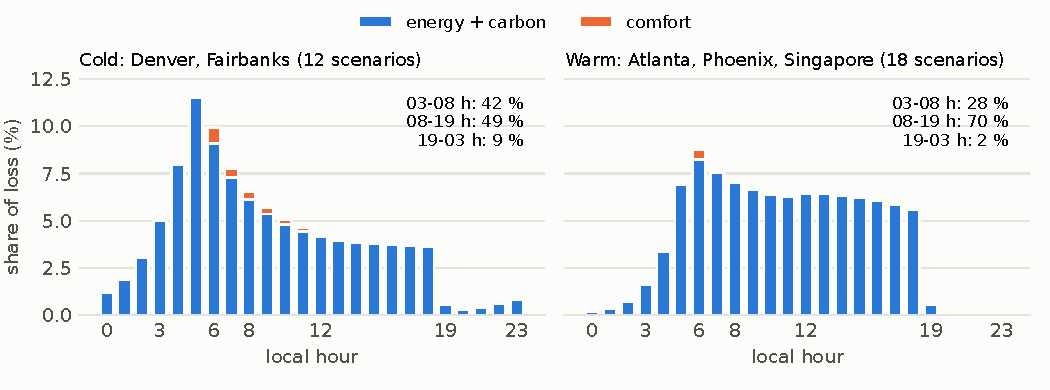
\includegraphics[width=\linewidth]{../docs/fig/fig_loss_hours.pdf}
\caption{Share of v11's training loss by local hour, cold stations (Fairbanks, Denver) and warm stations (Atlanta,
Phoenix, Singapore), split into energy plus carbon and comfort. 30 training scenarios, full length.}
\label{fig:hours}
\end{figure}

\subsection{Occupancy is visible in the heat balance, but not worth acting on}
% docs/TUNING_LOG.md (23 Oct, 12:00-13:34); sb/occ_dump.py, sb/occ_detect.py, sb/occ_detect2.py, sb/fig_occ.py.
The simulator adds 70\,W per person to the zone that person is in, comfort counts only in occupied zones, people
leave one by one from 13:00, and about 9\,\% of them never arrive on a given workday; only the building total is
observed. The controller reads only this total; it never replays the occupancy model, which the hosts have
ruled out. A controller that knew which zones are empty for the rest of the day could run them like zones at night.
The signal is real: averaged over 262 afternoon departures and 274 arrivals, the heat the controller gives a zone
rises or falls by about one person's 70\,W within three steps (Figure~\ref{fig:occ}). Zone by zone it is not
reliable: the zone that lost a person ranks first among the occupied zones in 26\,\% (Fairbanks) and 47\,\% (Phoenix)
of departures, against about 7\,\% by chance, below the 60\,\% we set before the test. Even perfect knowledge, from an
oracle that reads the simulator's occupancy (training only, never submitted), lowers the loss by only 2.6\,\% on eight
training scenarios, below the 5\,\% we set before the run. Comfort carries a large weight (one occupied zone 0.2\,K
outside its band costs about twice that zone's energy per step in Fairbanks), and the afternoon is a small part of the
loss. For the whole building one signal does pay: on holidays nobody comes in (Section~\ref{sec:holiday}); another participant raised the same holiday calendar
independently on the starter kit's issue tracker in November 2026 (issue 6), after our timestamped finding of 30 October.
\begin{figure}[t]\centering
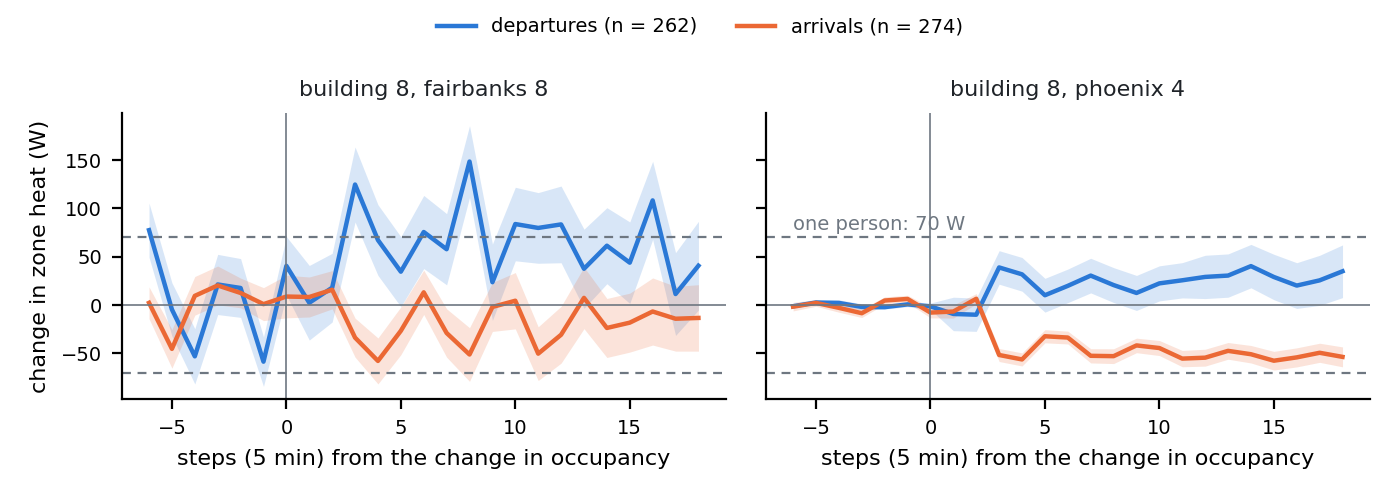
\includegraphics[width=\linewidth]{../docs/fig/fig_occ.png}
\caption{Change in the heat the controller gives a zone around the step in which a person leaves (blue) or arrives
(orange), relative to the other zones and to the zone's own six steps before; mean over events with one standard
error (building 8, seven days). Dashed: one person's 70\,W.}
\label{fig:occ}
\end{figure}

\section{New climates: details of the stress test}\label{app:stress}
% docs/STRESS_TEST.md (plan, rule, result, diagnosis); sb/make_stress.py, sb/stress_eval.py, sb/stress_diag.py,
% sb/stress_dump.py, sb/stress_dump2.py; results/stress, results/stressdiag.
The hidden test set uses five weather stations that appear nowhere in training, and our public scores have been
1.35--1.44 times our training scores, against 1.11 on our own round-5 buildings. Either the hidden climates are harder
for everyone, or our controller does worse in climates it has not seen. To test the second, we ran v13 and pid\_water
on the six training buildings with hourly 2023 weather for ten other cities (ERA5 reanalysis \cite{hersbach2020era5} through
Open-Meteo\footnote{\url{https://open-meteo.com}}; contains modified Copernicus Climate Change Service information: Miami, Houston, Las Vegas, San Francisco, New York, Seattle,
Chicago, Helena, Duluth and Dubai), converted to the shipped format, in two 30-day windows each (from 15 January and
from 15 July), 40 scenarios in all. The rule was fixed before the runs: if the ratio of mean losses v13/pid\_water
stays within 1.2 times its training value (0.136), the controller keeps its advantage; a city at 1.5 times or more is
a weak spot, to be diagnosed before any change.

v13 was better than pid\_water in all 40 scenarios, and the ratio of means was 0.143: by the rule, it keeps its
advantage in new climates. Three cold continental cities crossed the weak-spot mark: Chicago (0.236), Duluth (0.233)
and Helena (0.231). The training set has only three windows colder than 5\,$^\circ$C on average, all in Fairbanks;
the stress set has ten. In Chicago and Helena the diagnosis found no fault of ours: v13's energy per heating
degree-hour was at or below its training level and its comfort loss was near zero, while pid\_water, which loses
comfort all day there, happens to do relatively well in moderate cold.

Duluth exposed a real flaw in one building. In building 7, 28\,\% of the occupied zone-steps were below the band,
yet every box that missed was heating at the 35\,$^\circ$C cap with only about a fifth of its maximum airflow, and
no air handler was near its limit. The planner closes a damped fraction of the gap between a zone's no-heat trajectory
and its aim, so it also damps the heat that merely holds the zone against its losses. At equilibrium the zone then
sits about $(1-\mathrm{damping})/\mathrm{damping}$ times its one-step loss below its aim: about 0.41\,K predicted for one
zone at 4.8\,kW, 0.53\,K observed. The disturbance estimate cannot remove this offset, because it tracks the model's
one-step prediction error, which is near zero when the model is right, and not the distance from the aim. Under mild loads the heating margin absorbs this droop, which is why no training
run showed it; building 7's exterior zones lose heat three to six times faster than its median zone, and in deep cold
they fall out of the band. The fix (v14) leaves the damping in place but, in comfort time only, raises a goal
that would leave the comfort band to just inside it, so the tuned margins still absorb mild droop. Rules fixed
before the runs asked for no loss on the training set and a gain on the stress set: training 0.007328 against
0.007355 ($-0.37$\,\%), stress 0.007302 against 0.007398 ($-1.30$\,\%), with building 7 in Duluth $-5.3$\,\% and
its comfort regret down from 4.21 to $1.56\times10^{-3}$ per step.

\section{Simulator energy accounting}\label{app:tank}
% docs/TANKFIX.md; sb/make_tankfix.py, sb/tankfix_check.py; results/tankfix. Hosts' plan: Kaggle discussion 749531
% (host reply about 29 Oct, read 30 Oct; docs/PAPER_PLAN.md).
Participants have reported an accounting issue in the simulator's hot-water tank model on the competition forum, and
one has proposed a fix in which the tank follows an energy balance and gas is billed as the burner's heat (starter-kit
pull request~2\footnote{\url{https://github.com/smart-buildings-2026/starter-kit/pull/2}}). We wrote the same
equations into a copy of the simulator. With the setpoint held, the bill under the fix equals the shipped bill at
every step once the tank has heated from its initial 340\,K (a known-answer check in the repository). On the five
training scenarios of building 1, v13's score changes by at most 0.0002\,\%, against a mark of 0.1\,\% written before
the runs, while the official pid\_water baseline, which moves the setpoint, loses 34\,\% in Fairbanks. Our results do
not depend on the issue. The hosts aim to run the final leaderboard verification on a corrected simulator (forum,
October 2026).

% docs/FIXSIM.md; sb/make_fixsim.py, sb/run_fixsim.py; results/fixsim. Forum thread 753804, starter-kit PR 3.
A second issue was reported later: the air handler recirculates air at the floor-area mean of its zones, although each
zone exchanges heat at its own airflow, so the recirculated air can carry heat that no stream carried (starter-kit pull
request~3). We added the proposed airflow weighting to the same copy, in our own code. We then ran v16 and pid\_water
on six cold full-size development windows from 15 January (Chicago twice, Helena, Duluth, New York, Seattle) and six
hot ones from 15 July (Dubai, Las Vegas twice, Houston, Miami, Chicago), ten days each. The reading rule was written
before the runs: a change below 3\,\% counts as no dependence. v16's mean loss rises by 2.1\,\% in the cold windows (0.00924 to 0.00943; worst, Seattle,
$+4.3$\,\%) and 0.1\,\% in the hot ones. pid\_water moves by 2.1\,\% and 0.1\,\% on the windows with a shipped run, nearly
all of it in Duluth ($+20.8$\,\%). On the corrected copy v16 stays below pid\_water in all twelve windows (ratio of
means 0.23). This copy is our reading of the proposals, not the hosts' corrected simulator, which has not been published.

\section{Round 8: a delay-aware heating net}\label{app:r8}
% docs/HEATNET.md (exploration; screen rules written 31 Oct 13:00, result read 15:32); docs/PREREGISTRATION_8.md
% (stamped 31 Oct 15:33 local, before generation); docs/RESULTS_ROUND8.md (read 16:15).
v16 makes only the cooling safety net delay-aware, and in round 7's smallest rooms the heating net still gave full
effort on the lagged reading during the morning recovery. The candidate makes the heating net wait for the heat
already in the pipe as well (an existing option; no code change). It passed a screen with rules written before its
runs (training $-0.10$\,\%, no window more than 0.02\,\% worse; cold full-size windows $-0.08$\,\%; hot ones
unchanged) and went to round 8: six new full-size buildings, one ten-day window each, from Duluth at a mean of
$-15\,^\circ$C to San Francisco. Its loss was 0.12\,\% below v16's (mark 0.3\,\%: failed); it was at or below v16 in
five of six buildings and nowhere more than 0.01\,\% worse (both passed), with 3\,\% less comfort regret (passed).
Only Chicago gained ($-1.5$\,\%); Duluth carried two thirds of the summed loss and did not change. The plan had
predicted this outcome for a set with at most one building with small, fast rooms. The candidate is harmless, but its
gain is too rare to pay on average, so v16 stays.

\section{Faulty sensors}\label{app:faults}
% docs/SENSOR_FAULTS.md (rules written 4 Nov 2026 16:25 and stamped before any run; result read 6 Nov 01:00);
% policies/zonal_v16_faults.py, sb/run_faults.py.
The simulator's sensors are perfect; a real building's are not, and the organisers plan to evaluate winning solutions
on real buildings after the contest \cite{goldfeder2026smart}. We fed the frozen v16 zone temperatures through five
faults while the simulator's true temperatures still set the comfort term, on the twelve full-size buildings of
rounds 6 and 7 (seen before, so post hoc; ten days each). With no fault the wrapper reproduces v16 exactly. Rules were
written and timestamped before the runs (Appendix~\ref{app:stamps}): ordinary noise should cost at most 10\,\%, one extra step of delay at most 25\,\%, and with
10\,\% of the zone sensors dead v16 should stay below pid\_water (with perfect sensors) in at least ten of twelve (Table~\ref{tab:faults}).

\begin{table}[!htb]\centering
\caption{Sensor faults on the twelve full-size buildings of rounds 6 and 7, ten days each. Loss relative to v16 with clean sensors; worst: the largest ratio over the twelve; below pid\_water: buildings in which faulty v16 stays below pid\_water with perfect sensors.}\label{tab:faults}
\small
\begin{tabular}{lcccc}
\toprule
fault & loss / clean v16 & worst & comfort term & below pid\_water \\
\midrule
none (clean) & 1 & -- & 0.00048 & 12 of 12 \\
noise, 0.2\,K per step & 1.01 & 1.05 & 0.00072 & 12 of 12 \\
noise, 0.5\,K per step & 1.08 & 1.26 & 0.00140 & 12 of 12 \\
fixed bias per zone, 0.5\,K s.d. & 1.36 & 2.14 & 0.00533 & 12 of 12 \\
one more step of delay & 1.50 & 2.34 & 0.00436 & 12 of 12 \\
10\,\% of zone sensors stuck & 2.30 & 8.15 & 0.01449 & 10 of 12 \\
\bottomrule
\end{tabular}
\end{table}

Noise passed (1.01): learning online does not make the controller fragile to ordinary sensor noise. The extra delay
failed (1.50): the safety net waits for exactly one step, so with two it acts late, worst in hot, humid windows
($\times$2.2--2.3), and the comfort term grows ninefold. Dead sensors passed at the mark (10 of 12; the two misses are
hot windows where pid\_water itself is cheap): a stuck zone is simply not controlled, so the loss is mostly comfort, and
the relative cost is largest where v16 is cheapest. In 58 of 60 faulty runs v16 stays below pid\_water with perfect
sensors. Before a real deployment, then, the reading delay has to be measured on site (the probe of
Appendix~\ref{app:probe} does this), and dead sensors have to be detected, for instance a zone whose reading does not
move while its damper and reheat do.

Measuring the delay is only useful if setting it helps. After these runs we therefore added one option to the v16
file: the extra delay in steps, $d$. The controller then learns from the heat sent $d$ steps further back, and before
it plans it rolls its zone model forward through the heat already sent. The safety nets act on the rolled-forward
temperature, and cool-hold stays at two steps. With $d=0$ the option reproduces v16 exactly. Rules were written
before the runs (\texttt{docs/LAG\_SETTING.md}): at most 1.25$\times$ clean v16, and better than unaware v16 in at least
10 of 12 buildings. With one extra step of delay and the setting $d=1$, the loss is 1.00$\times$ clean v16 (worst
1.01$\times$, comfort 0.00046 against 0.00436), better in 12 of 12. A wrong setting ($d=1$ with no extra delay) costs
1.27$\times$ (worst 1.47$\times$), so the probe matters in both directions. This is a post-hoc test on buildings we had
seen; v16 as submitted is unchanged.

\section{Ablations}\label{app:abl}\label{sec:abl}
% sb/fig_transfer_abl.py; docs/TRANSFER_ABLATION.md (day-by-day ratios: sb/run_transfer_abl.py --days).
\begin{figure}[t]\centering
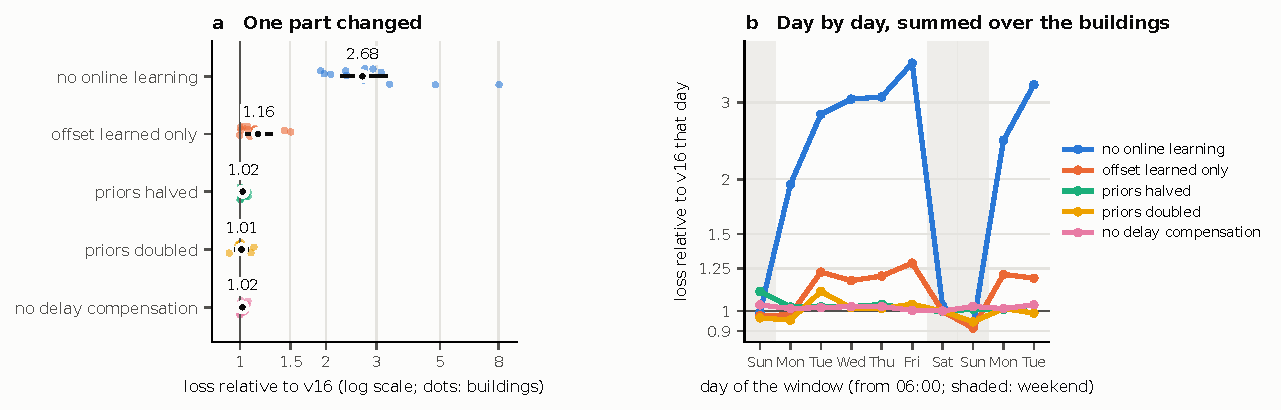
\includegraphics[width=\linewidth]{../docs/fig/fig_transfer_abl.pdf}
\caption{What carries the transfer (Section~\ref{sec:what}, Table~\ref{tab:what}). (a) Each variant's loss relative
to v16 in each of the twelve full-size buildings of rounds 6 and 7 (dots), and the ratio of means with its 95\,\%
bootstrap interval. (b) Day by day, the variant's loss summed over the buildings relative to v16's; every window
starts on a Sunday at 06:00, and comfort counts only on work days.}
\label{fig:what}
\end{figure}
\textbf{v16.} Without online learning the gap opens on the first work day and widens through the week
(Figure~\ref{fig:what}b). With halved priors the first day costs 11\,\%; from the second day on the variant stays
within 4\,\% of v16. Without delay compensation the loss is 1--3\,\% higher on eight of the ten days and within
0.3\,\% of v16's on the other two.

% docs/COLD_START.md (rules 8 Nov 23:36, before any run; read 9 Nov 00:03); sb/run_coldstart.py --read.
\textbf{Cold start on a work day.} Most windows start on a weekend, so the controller runs for a day or two before
comfort first counts. For a true cold start we re-created v16 from nothing (every learned number at its starting value,
no memory of earlier steps) at 06:00 on the first work day of the twelve full-size windows of rounds 6 and 7, with the
reading rules timestamped before the runs (post hoc, as above). The 288 steps from the restart cost 1.20 times v16's
loss on the same steps (95\,\% interval over buildings 1.09--1.34; per building 1.05--1.83, worse in all twelve). By the
rule written in advance that is a modest cost, so we no longer claim that the first work day costs nothing. The whole
rise is comfort: the comfort term summed over the twelve goes from 5.1 to 21.3 while the total loss goes from 75.9 to
90.8. The restarted controller stays below pid\_water in all twelve on that day (median ratio 0.24, against 0.22 for
v16), and the next 288 steps cost 1.01 times v16's (interval 0.99--1.04). Before the restart each run matches v16 step for
step, so the building arrives in the state that v16's own weekend left it in; this is not a hand-over from another
controller.

% docs/TRANSFER_ABLATION2.md (rules 8 Nov 19:05, before any run; read 23:37); sb/run_transfer_abl2.py --read.
\textbf{What the delay and the slab are worth.} Table~\ref{tab:what} left two questions open: planning past the delay
was switched off alone, while two other responses to the same lag stayed on, and the slab node stayed on in every
variant. We ran five more variants on the same twelve buildings and steps, with the reading rules timestamped before
the runs (Table~\ref{tab:what2}; post hoc, as before). The rules give four readings, each with its mark in brackets.
All the delay handling together carries a large part of the transfer (at least 10\,\% worse, interval above 1, worse
in at least 10 of 12). The overlap that Section~\ref{sec:what} describes holds (ratio at least 1.04). The slab node
matters (at least 5\,\% worse, interval above 1). The slab's lag need not be exact (each within 5\,\%, no scenario
more than 15\,\% worse). The rise without any
delay handling is concentrated: four buildings carry it (New York in October $+119$\,\%, Duluth in December $+58$\,\%,
Chicago in December $+48$\,\%, New York in January $+19$\,\%), and in the other eight the change is at most $+2$\,\%.
The rule against cooling right after heating never fires in nine of the twelve buildings. A two-hour slab lag is
0.8\,\% below v16's on the mean, with an interval that includes 1; v16 did not change.
% docs/PUBLIC_ABLATION2.md (rules written and timestamped before any build; scores read 10 Nov, 07:31 UTC).
On the public leaderboard (Table~\ref{tab:what2}, last column; rules fixed before submission) the score with all the
delay handling off is 1.23 times v16's. So the delay handling carries a large part of the transfer on the hidden
buildings too. Without the slab node the score is 1.78 times v16's: the slab matters there as well. With a two- or
eight-hour lag it is 1.00 and 1.01 times, so the lag need not be exact there either. Without the cooling rule it is
1.00 times.
\begin{table}[!htb]\centering
\caption{More variants of v16, as in Table~\ref{tab:what} (all delay handling off: planning past the delay, the delay-aware
safety net and cool-hold): mean loss relative to v16's with a 95\,\% bootstrap interval over buildings. Worse in: buildings in which the variant's loss is higher (without the cooling rule the other nine are identical runs; with a two-hour lag the other seven are better). Public: Kaggle public score relative to v16's 0.01031 (one score
each).}\label{tab:what2}
\small
\begin{tabular}{lcccc}\toprule
Variant of v16 & Loss / v16 & Worse in & Comfort & Public\\\midrule
v16 & 1 & -- & 0.00048 & 1\\
all delay handling off & 1.14 (1.03--1.30) & 12 of 12 & 0.00173 & 1.23\\
no cool-hold rule & 1.05 (1.00--1.12) & 3 of 12 & 0.00099 & 1.00\\
no slab node (three-number model) & 1.16 (1.09--1.27) & 12 of 12 & 0.00189 & 1.78\\
slab lag two hours instead of four & 0.99 (0.98--1.00) & 5 of 12 & 0.00040 & 1.00\\
slab lag eight hours & 1.02 (1.01--1.03) & 12 of 12 & 0.00062 & 1.01\\\bottomrule
\end{tabular}
\end{table}

% docs/TUNING_LOG.md (23 Oct, ablations of v11); docs/RESULTS_EXTERNAL.md (public scores of two ablations).
\textbf{v11.} Removing one part of v11 at a time (Table~\ref{tab:abl11}): without the slab node the loss doubles and
comfort regret grows 32-fold, because the other parts rely on predictions only the slab model gets right. The pump
pressure reset and the cooling setback are each worth 6--8\,\%, and their public ratios to v11 (1.058 and 1.077) match
the training ratios (1.064 and 1.079), so both carry over to the hidden test set.
\begin{table}[h]\centering
\caption{Ablations of v11, one change each. Training: 30 scenarios, full length. Public: the public leaderboard
(about a third of the hidden test set); only the first two variants were submitted, for this table only, never used for tuning.}\label{tab:abl11}
\small
\begin{tabular}{lccccc}\toprule
Variant & Training & / v11 & cold / warm & Public & / v11\\\midrule
v11 & 0.00744 & 1 & 1 / 1 & 0.01071 & 1\\
without pump pressure reset & 0.00792 & 1.064 & 1.095 / 1.030 & 0.01133 & 1.058\\
without cooling setback & 0.00802 & 1.079 & 1.013 / 1.152 & 0.01153 & 1.077\\
without slab node & 0.01524 & 2.048 & 1.600 / 2.550 & -- & \\\bottomrule
\end{tabular}
\end{table}
% Numbers from D:/SmartBuildings_data/results/dev_2880/<folder> via sb.compare (16 Oct 2026).
\textbf{The first controller.}
On the six-scenario, ten-day development set (Table~\ref{tab:abl}), online identification and the cost-based
supply-air setpoint matter most; without either, the loss doubles. Two components did not help there: delay
compensation and idle-zone reheat. Per scenario, delay compensation helps Denver~2 and Atlanta~8, makes no difference
in Fairbanks~1 and hurts the cooling-dominated Phoenix~6, Singapore~4 and Denver~6. They were kept because the
controller had been frozen before the ablations ran. Once the limit cycle of round 1 was removed, delay compensation
helped (the v8 rows of Table~\ref{tab:abl}); we read its apparent cost in v7 as an interaction with that cycle.
\begin{table}[h]\centering
\caption{Ablations on the development set (six training scenarios, ten days).}\label{tab:abl}
\small
\begin{tabular}{lc}\toprule
Variant & Dev score\\\midrule
Full controller (v7, frozen) & 0.02305\\
No online identification (fixed $g,\lambda$) & 0.05028\\
No cost-based supply-air setpoint & 0.04895\\
No heating airflow cap & 0.02400\\
Cooler hot water (330/310\,K) & 0.02338\\
No idle-zone reheat & 0.02202\\
No delay compensation & 0.02120\\\midrule
v8 (cooling-only net fix + disturbance estimate) & 0.01893\\
Disturbance estimate only & 0.01940\\
v8 without delay compensation & 0.02011\\\midrule
pid\_water baseline & 0.10156\\\bottomrule
\end{tabular}
\end{table}

\section{Full-size buildings: hot load and cold recoveries}\label{app:monday}
% sb/bigbld_dump.py traces (results/bigbld_diag), sb/size_parts.py; docs/BIG_BUILDINGS.md (29 Oct: room left).
% Occupied-hours cooling share of the extra loss: +0.0089 of +0.0100 per step; +0.0096 of +0.0106 in the replication.
\textbf{Hot weather: the load, not a fault.} In Dubai v14's loss nearly doubles at full size: the building has 2.15
times the floor area on the same four air handlers, and energy is normalised per air handler. Per square metre v14
cools with 12\,\% less power and still holds comfort; about 90\,\% of its extra loss is the cooling bill of occupied
hours, with the supply air at its coldest setpoint, the static pressure at the simulator's floor on three of four air
handlers and the rooms 0.1\,K inside the band. If the hidden buildings are full size, hot scenarios weigh more in
public than in training, for every team.

\textbf{Cold weather: recoveries in large rooms.} In the building with the largest rooms (850--890\,m$^2$, on the same
2\,m$^3$/s box as every other zone), the comfort loss sits on one Monday morning after a cold weekend: the slab holds
their recovery to about 0.7\,K/h, a third of the rate our setback (Eq.~\ref{eq:glide}) assumes
(Figure~\ref{fig:monday}). Shipped buildings have large boxes for their rooms, so no earlier run showed it.

% sb/fig_monday.py; results/bigbld_diag/v14_7407_chicago_full_d8.npz and v15A_7407_chicago_full_d8.npz.
\begin{figure}[t]\centering
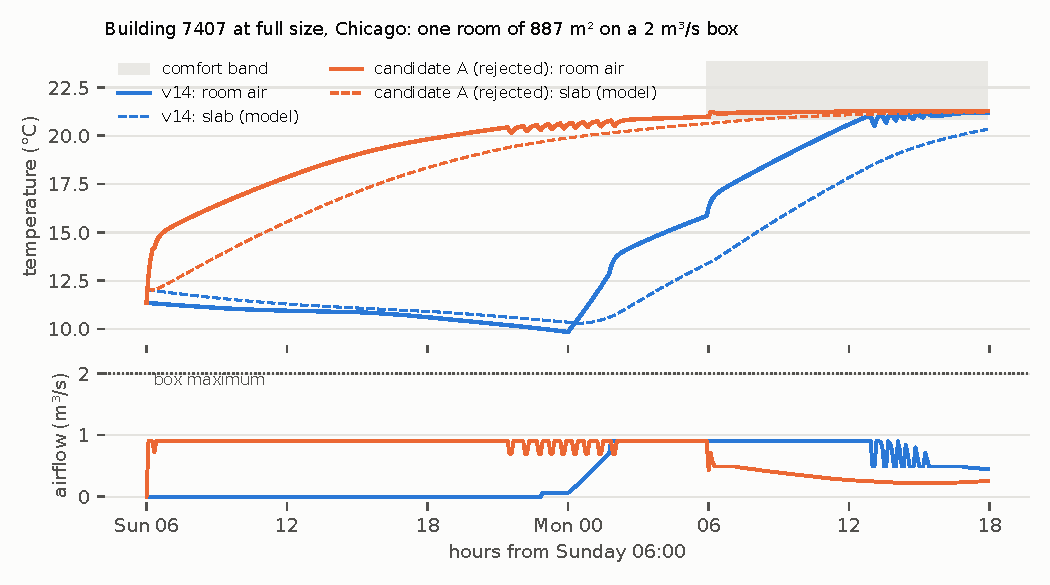
\includegraphics[width=\linewidth]{../docs/fig/fig_monday.pdf}
\caption{The largest room (887\,m$^2$) of building 7407 at full size, Chicago, after a cold weekend. v14 (blue) lets
the room float to 9.8\,$^\circ$C, starts heating shortly before midnight, and reaches the band 6.6 hours after the
comfort period begins, at the pace of the slab. The rejected candidate A (orange) heats from Sunday morning and is on
time, but the building's loss over these 36 hours is 14\,\% higher.}
\label{fig:monday}
\end{figure}
% docs/BIGDEV.md (candidates, screen and full-check rules, timestamped 25 Oct; screen results 27 Oct);
% results/bigdev/<candidate>/*.json and *.npy; sb/v15_screen_eval.py. Deep cold: docs/V15COLD.md (rules 30 Oct
% 00:46 and 00:52; stage 1 decided 30 Oct), results/v15cold, frozen/zonal_v15dev_h.py; simulator vav.py.
Two fixes were screened, with candidates and rules fixed before the runs (mean loss 1--2\,\% lower, no scenario 2\,\%
worse). In mild weather, letting the setback assume the slower, slab-limited rate fixed Monday (comfort regret
$-94$\,\%), but the large rooms then started heating a day early and the loss rose by 18\,\%. In deep cold the large
rooms are held back by the heating airflow cap instead. Six variants that raise it, plainly or priced against comfort,
lost on their first scenario ($+3$ to $+44$\,\%), and comfort got worse in every one. The static pressure is shared and
no damper closes below 10\,\%, so a higher cap for one room pushes air at about 8\,$^\circ$C through every other box.

\section{One-parameter sensitivity at full size}\label{app:sens}
% docs/FULLSWEEP.md (variants and rule fixed 30 Oct 01:48, before any run; result read 30 Oct 10:01, with the split by
% reward term); sb/run_fullsweep.py --read; results/fullsweep, reference results/bigdev/v14. Scaled-size result for
% the later recovery start: docs/TUNING_LOG.md, screen b (23 Oct).
v14's parameters were tuned on scaled buildings. To check that they still sit near an optimum at full size, we moved
five of them one at a time (three both ways) on four full-size development scenarios (two hot, two mild cold; 2880
steps each), with the
rule fixed before the runs: a change counts if the mean loss falls by at least 1\,\% and no scenario is 2\,\% worse.
None did (Table~\ref{tab:sens}). Raising the heating airflow cap changes almost nothing; lowering it costs a little in the cold. In hot weather every change that acts there
lost 0.4--1.5\,\%. In the cold windows, changes that heat less lower the loss by up to 2.1\,\%, trading a little
comfort for energy, and the opposite changes raise it.

% Slope of log gain on log area: docs/PARAMS.md (sb/params_read.py on the size-gate traces, read 31 Oct 03:35).
% docs/SIZEGATE.md (diagnostic, sb/sizegate_read.py; upside check read 30 Oct 18:26), docs/HEATLESS.md (rule 30 Oct
% 18:17, before any run; result read 30 Oct, sb/run_screen_m.py --read; per-day split of building_train_8 atlanta_1).
On scaled buildings in deep cold, though, the later recovery start had cost 5.4\,\% (three of four training
scenarios). A rule that knows the building's size seemed the way out, and the controller's own zone models do see room
size: after three days a zone's learned gain per kW falls as its room grows (rank correlation of its inverse with room
area 0.63--0.82 within each full-size building). Over all 17 traced buildings (1187 zones, none at a bound), the
within-building slope of log gain on log area is $-0.32$ (95\,\% interval over buildings $-0.39$ to $-0.24$,
$R^2=0.46$) and negative in every building, though far from the $-1$ of a gain inversely proportional to the room's
heat capacity. Here $q$ is the box's sensible heat in kW, and box size does not scale with floor area in the generator,
so we read the slope as a description of these buildings, not as an estimate of heat capacity. But heating less paid in small rooms too. A smaller margin together
with the later start lowered the loss in all six cold full-size development windows ($-1.5$ to $-4.9$\,\%), most in
mild Seattle and in a building of small rooms, so a size rule had nothing to stand on. We then screened the smaller
margin alone (0.30\,K), with its rule fixed before the runs: mean at least 1\,\% lower in the six cold full-size
windows, total at most 0.1\,\% higher over the 30 training scenarios at full length, and no scenario 2\,\% worse in
either. It lowered the loss by 1.6\,\% in all six windows and by 0.3\,\% over the training scenarios, but one mild
Atlanta window lost 4.4\,\%, all of it on its first Monday, when the comfort regret was 5.5 times v15's. So v15 keeps
its margin.

\begin{table}[h]\centering
\caption{Change of the loss (\%) over 2880 steps when one parameter of v14 is moved, on four full-size development
scenarios. Heating-only changes, identical to v14 in Dubai, were not run in Las Vegas (--, counted at v14's loss). Mean: change of the mean loss over the four scenarios, a ratio of means, so each scenario weighs by its loss and the two hot scenarios dilute a heating-only change.}
\label{tab:sens}
\small
\setlength{\tabcolsep}{4pt}
\begin{tabular}{llrrrrr}
\toprule
parameter & v14 $\to$ & Dubai & Las Vegas & Chicago & New York & mean \\
\midrule
heating airflow cap (of box max.) & 0.245 $\to$ 0.316 & 0.00 & -- & $+0.01$ & $-0.04$ & 0.00 \\
 & 0.245 $\to$ 0.20 & 0.00 & -- & $+0.09$ & $+0.13$ & $+0.03$ \\
glide safety factor $\alpha$ & 0.66 $\to$ 0.50 & 0.00 & -- & $+1.05$ & $+2.83$ & $+0.56$ \\
 & 0.66 $\to$ 0.80 & 0.00 & -- & $-0.09$ & $-1.45$ & $-0.20$ \\
damped fraction per step & 0.74 $\to$ 0.90 & $+1.30$ & $+1.11$ & $+2.12$ & $+2.73$ & $+1.59$ \\
 & 0.74 $\to$ 0.60 & $+0.93$ & $+0.40$ & $-1.90$ & $-2.07$ & $-0.13$ \\
cooling glide safety factor & 0.55 $\to$ 0.70 & $+1.50$ & $+0.58$ & $-0.01$ & $-0.06$ & $+0.78$ \\
heating margin (K) & 0.40 $\to$ 0.30 & 0.00 & -- & $-1.49$ & $-1.66$ & $-0.50$ \\
\bottomrule
\end{tabular}
\end{table}

\section{Control step and settings of v16}\label{app:settings}
% frozen/README.md (reproduction check, 30 Oct 2026); sb/repro_check.py. docs/TUNING_LOG.md (30 Oct, compute per
% step); sb/timing.py.
Runs are deterministic (a frozen version reproduced a recorded 30-day run exactly), and the controller takes a median
of 0.6\,ms per step on one laptop core, under 2\,\% of the simulator's time; the competition caps a rollout at ten times
the bang-bang baseline's run time \cite{goldfeder2026smart}.

% Copied from submission/V16_PARAMS.json and the comments of frozen/zonal_v16f.py (8 Nov 2026).
% Algorithm 1 follows TransferPolicy.get_action in frozen/zonal_v16f.py with the V16_PARAMS.json settings (8 Nov 2026):
% _identify_m2 (err_clip 0.5, m2_lo/m2_hi, p_trace_max 1, dist_beta 0.1, dist_max 1.5, mass_n 48); lead_h 2 (24 steps);
% guard 1; offset_free 3 (only when h2c == 0); safety_k 1.5 with safety_pred 2 (t1 gate on cooling only); cool_hold 2;
% sat_econ candidates sat_min 285 K in sat_econ_step 1 K up to min(0.7 T_ret + 0.3 T_oa, sat_econ_max); _plan_ahu cost;
% pfrac = max(max flow fraction^2, 0.1) (200 Pa floor); water_heat = water_idle = 350 K; dp_reset 2.
Algorithm~\ref{alg:step} lists one control step, Table~\ref{tab:settings} the settings v16 passes to the frozen
code, and Table~\ref{tab:numbers} the numbers and formulas that are the code's defaults. The same settings run in
every building. Temperatures in K; v16 identifies only the model of Eq.~\ref{eq:m2}, by recursive least squares with
a forgetting factor of 0.998 (the first-order model of earlier versions is not used).
\begin{algorithm}[H]
\caption{One five-minute control step of v16, for all zones $z$ at once (Sections~\ref{sec:model}--\ref{sec:schedule}).
Numbers are the settings of Table~\ref{tab:settings}, rounded; airflow caps are fractions of each box's maximum.}\label{alg:step}
\small\raggedright
\begin{algorithmic}[1]
\Require zone temperatures $T_{z,k}$, outside temperature, comfort flag, occupant count, clock
\State Update each zone's five numbers in Eq.~\ref{eq:m2} by recursive least squares on the step that just ended
(error clipped at 0.5\,K, parameters bounded, covariance trace at most 1); update the disturbance estimate $\hat d_z$
(a smoothed model error) and the slab node $T^m_z$
\State $N_k \gets$ steps until the comfort period (0 inside it); if nobody has come in an hour after the comfort
period starts, the day runs as unoccupied until someone arrives
\If{$N_k \le 24$}
\State $[\ell_z,u_z] \gets$ the comfort band narrowed by 0.30\,K (heating side) and 0.25\,K (cooling side)
\Else
\State $[\ell_z,u_z] \gets$ the eco band narrowed by 1\,K
\EndIf
\If{$N_k>0$}
\State $\ell_z \gets$ the floor of Eq.~\ref{eq:glide} (heating season only); $u_z \gets$ its cooling mirror; both replace the band set above
\EndIf
\State $\hat T_{z,k+1} \gets$ Eq.~\ref{eq:m2} with the heat already in the pipe, plus $\hat d_z$
\State $\hat T^{0}_{z,k+2} \gets$ Eq.~\ref{eq:m2} from $\hat T_{z,k+1}$ with no new heat, plus $\hat d_z$
\For{each zone with $\hat T^{0}_{z,k+2}$ outside $[\ell_z,u_z]$}
\State aim $a_z \gets \ell_z+0.08$ (or $u_z-0.08$)
\State goal $\gamma_z \gets \hat T^{0}_{z,k+2}+0.74\,(a_z-\hat T^{0}_{z,k+2})$; in the comfort period at least
0.08\,K inside the comfort band
\State heat to deliver $q^{*}_z \gets (\gamma_z-\hat T^{0}_{z,k+2})/g_z$ (zero for the other zones)
\EndFor
\State Safety net: the most heat the airflow cap allows if $T_{z,k}<\ell_z-1.5$; full cooling airflow if both
$T_{z,k}$ and $\hat T_{z,k+1}$ exceed $u_z+1.5$; no cooling in a zone asked for heat in the last two steps
\For{each air handler}
\State Off if none of its zones needs heat or cooling. Otherwise, for each supply-air setpoint from 285\,K in 1\,K
steps up to the mixed-air temperature (at most 295.3\,K; none if no zone needs cooling), plan the box airflows and
estimate the cost in reward units (fan and chiller electricity, reheat gas, unmet cooling); keep the cheapest plan
\State Heating boxes discharge at 35\,$^\circ$C with airflow cap 0.245 (0.45 if more than 0.25\,K below the band; at
least 0.35 while unoccupied in the heating season); idle zones get the minimum airflow, with reheat if even
that would over-cool them
\State Static pressure from the most open damper (at least 200\,Pa)
\EndFor
\State Hot water at 350\,K; pump pressure the lowest at which every open reheat coil reaches its discharge
temperature, each reheat valve opened only as far as its coil needs; pump off if no zone is heated
\State \Return the actions; keep the planned heat $q_{z,k}$ of the final box plan (the next step's prediction uses it, and the identification one step later)
\end{algorithmic}
\end{algorithm}
\begin{table}[H]\centering
\caption{Settings of v16 (\texttt{submission/V16\_PARAMS.json}). Switches: 0 is off.}\label{tab:settings}
\footnotesize
\begin{tabular}{llp{0.54\linewidth}}\toprule
Setting & Value & Meaning\\\midrule
\texttt{mass\_model} & 1 & zone model with a slow mass node, an envelope term and an internal-gain term\\
\texttt{m2\_rate} & 1 & glide heating and cooling rates taken from the mass model\\
\texttt{dist\_obs} & 1 & offset-free prediction with a per-zone disturbance estimate\\
\texttt{offset\_free} & 3 & droop fix: in the comfort period, a goal outside the comfort band moves to just inside it (App.~\ref{app:stress})\\
\texttt{safety\_pred} & 2 & full cooling effort only if the zone stays far out after the heat already in the pipe\\
\texttt{cool\_hold} & 2 & steps after a zone was last asked for heat in which it is not cooled\\
\texttt{margin\_heat}, \texttt{margin\_cool} & 0.3, 0.25 & aim this far inside the heating and cooling setpoints\\
\texttt{aim\_inside} & 0.079 & further inside the band when the controller must act\\
\texttt{damping} & 0.7445 & fraction of the gap to target closed per step\\
\texttt{f\_heat\_max} & 0.2453 & heating airflow cap, fraction of the box maximum\\
\texttt{f\_heat\_safety}, \texttt{boost\_k} & 0.45, 0.25 & higher cap for zones more than \texttt{boost\_k} below their band\\
\texttt{f\_heat\_rec} & 0.35 & heating airflow cap while unoccupied\\
\texttt{night\_glide} & 1 & unoccupied heating floor that rises towards comfort at the rate the zone can heat\\
\texttt{glide\_floor} & $-16$ & lowest floor, relative to the eco band's lower edge\\
\texttt{glide\_safety} & 0.6606 & fraction of the identified heating rate the glide assumes\\
\texttt{glide\_oat} & 291.45 & glide only while the 24-hour mean outside temperature is below this\\
\texttt{cool\_glide} & 1 & unoccupied cooling ceiling that falls towards comfort at the zone's pull-down rate\\
\texttt{cool\_ceiling} & 8 & warmest ceiling, relative to the eco band's upper edge\\
\texttt{cool\_safety} & 0.55 & fraction of the identified cooling rate the path assumes\\
\texttt{sat\_econ\_max} & 295.3467 & upper limit on the supply-air setpoint when mixing outside air\\
\texttt{dp\_reset} & 2 & hot-water pump pressure reset, each reheat valve opened only as far as its coil needs\\
\texttt{empty\_day}, \texttt{empty\_h} & 1, 1.0 & a workday with nobody in 1 h after comfort start runs as unoccupied\\\bottomrule
\end{tabular}
\end{table}

\begin{table}[H]\centering
\caption{Numbers and formulas of v16 that are defaults of the frozen code. Zone subscripts are dropped; $\dot V$ is airflow in m$^3$/s, $\bar T$ the mean zone temperature, $T^{w}$ the hot-water temperature, 1.206 the volumetric heat capacity of air in kJ/(m$^3$\,K).}\label{tab:numbers}
\footnotesize
\begin{tabular}{p{0.16\linewidth}p{0.78\linewidth}}\toprule
Quantity & Value or definition\\\midrule
Starting values & $(\lambda,g,c,b,c^{\mathrm{cm}})=(0.33,\,0.27,\,0.09,\,0.016,\,0.25)$\\
Bounds & $\lambda\in[0.05,0.8]$, $g\in[0.05,0.8]$, $c\in[-2,1.5]$, $b\in[0,0.12]$, $c^{\mathrm{cm}}\in[-0.5,1]$; every update is clipped to them\\
One-step error & $e=T_k-T_{k-1}-\phi^{\top}\theta$, with $\theta=(-\lambda,g,c,b,c^{\mathrm{cm}})$ and $\phi=(T_{k-1}-T^{m}_{k-1},\,q_{k-2},\,1,\,T^{\mathrm{oa}}_{k-1}-T_{k-1},\,\mathbf{1}_{\mathrm{comfort},k-1})$\\
Least squares & $P_0=\mathrm{diag}(10^{-3},10^{-3},10^{-2},10^{-5},10^{-2})$; forgetting 0.998; $e$ clipped to $\pm0.5$\,K; if $\mathrm{tr}\,P>1$ then $P\gets P/\mathrm{tr}\,P$\\
Disturbance estimate & $\hat d\gets\mathrm{clip}(0.9\,\hat d+0.1\,e,\,\pm1.5\,\mathrm{K})$, starting at 0, using $e$ before its clipping and before the parameter update\\
Slab node & $T^{m}$ starts at the first reading and follows Eq.~\ref{eq:m2}; the 48 steps are fixed, not learned\\
Prediction & $\hat T_{k+1}$ uses $q_{k-1}$; $\hat T^{0}_{k+2}$ uses no new heat and the slab rolled one step forward; outside temperature and comfort flag are held\\
Heat $q_k$ & $1.206\,\dot V\,(T^{\mathrm{dis}}-\hat T_{k+1})$ kW from the final box plan after all caps, negative when cooling\\
Recovery rate $\hat r$ & net one-step change of Eq.~\ref{eq:m2} plus $\hat d$, comfort flag 0, at airflow $0.35\,\dot V_{\max}$ and discharge $\min(35\,^\circ\mathrm{C},\,T^{s}+0.9(T^{w}-T^{s}))$ with $T^{s}=0.7\bar T+0.3T^{\mathrm{oa}}$; clipped to $[0.01,0.25]$\,K per step\\
Heating floor & Eq.~\ref{eq:glide} less than 24\,h before the comfort period; further away $T_{\mathrm{eco}}-\Delta$\\
Cooling ceiling & $\min(T^{\mathrm{eco}}_{\mathrm{hi}}+8,\ T^{*}_{c}+0.55\,\hat r_{c}\max(N_k-2,0))$ less than 24\,h before the comfort period; further away $T^{\mathrm{eco}}_{\mathrm{hi}}+8$. $T^{*}_{c}$: the comfort band's upper edge minus 0.33\,K; $\hat r_{c}$: net cooling rate of Eq.~\ref{eq:m2} with air at 285\,K at $\dot V_{\max}$, clipped to $[0.01,0.25]$\,K per step\\
Mixed air & for a supply-air setpoint $s$: recirculation $r=\min(0.7,\max(0,(s-T^{\mathrm{oa}})/(\bar T-T^{\mathrm{oa}})))$ if $T^{\mathrm{oa}}<\bar T-0.5$\,K, else 0.7; $T^{\mathrm{mix}}=r\bar T+(1-r)T^{\mathrm{oa}}$; supply air $T^{a}=\min(T^{\mathrm{mix}},s)$. With no cooling demand $r=0.7$ and no chilling\\
Duct pressure & $\pi=\max(\max_j(\dot V_j/\dot V_{\max,j})^2,\,0.1)$, as a fraction of 2000\,Pa; dampers $\mathrm{clip}(\dot V_j/(\dot V_{\max,j}\sqrt{\pi}),\,0.1,\,1)$\\
Cost estimate & fan $=2000\,\pi\,\dot V_{\mathrm{tot}}(2-r)/(0.9\cdot1000)$ kW; chiller $=1.206\,\dot V_{\mathrm{tot}}\max(0,T^{\mathrm{mix}}-T^{a})/3.5$ kW; gas $=1.206\sum_{\mathrm{reheat}}\dot V_j(T^{\mathrm{dis}}_j-T^{a})$ kW; unmet cooling $U=\sum_{\mathrm{cooling}}g_j\max(0,\,1.206\,\dot V_j(T^{a}-\hat T_{k+1,j})-q^{*}_j)$ K; cost $=[0.0023(\mathrm{fan}+\mathrm{chiller})+0.00105\,\mathrm{gas}]/n_{\mathrm{AHU}}+0.12\,U/n_{z}$\\
Pump pressure & for each open coil, $\varepsilon_j=(T^{\mathrm{dis}}_j-T^{a})/(T^{w}-T^{a})$ and $\rho_j=1.3\,\varepsilon_j\dot V_j\,1206\cdot3600/(0.108\cdot1000\cdot4180)$; pressure $\mathrm{clip}(\max_j\rho_j^2,\,0.5,\,20)$ bar (20 if some coil cannot reach its discharge temperature); valve opening $\min(1,\max(0.05,\rho_j/\sqrt{\text{pressure}}))$\\\bottomrule
\end{tabular}
\end{table}

\section{Frost protection}\label{app:frost}
% docs/FROST.md (rules written 7 Nov 2026 19:05, before any run; result read 8 Nov 00:22); policies/zonal_v16frost.py,
% sb/make_v16frost.py, sb/run_frost.py.
The simulator does not model freezing, and v16's night glide lets an empty zone float down to about 0\,$^\circ$C. The
hosts asked papers to report a frost limit and its cost. We added one option to the frozen v16, a floor under every
zone's heating setpoint (off by default; with it off the controller reproduces v16 exactly), and ran it at 5\,$^\circ$C
on the 21 cold windows of rounds 6--8 and our development set (2880 steps), plus six on a copy of the simulator with
both proposed energy fixes, with the reading rule fixed before the runs. Without the floor, v16's coldest zone over the
21 windows reached $-1.68\,^\circ$C (round 8, Duluth, 29 January); 7 windows went below 5\,$^\circ$C and 2 below
0\,$^\circ$C, and 0.80\,\% of zone-steps were below 5\,$^\circ$C (0.13\,\% below 0\,$^\circ$C). With the floor, every
window stayed above 0\,$^\circ$C, but the rule's mark (no zone below 4\,$^\circ$C) failed in two: Duluth reached
2.93\,$^\circ$C and New York (29 January) 3.29\,$^\circ$C, because a floor on the setpoint is not a floor on the
temperature when heating lags and is at its limit. The floor raised the loss by 0.70\,\% over the 21 windows (worst
3.6\,\%, Duluth; 14 windows never reach 5\,$^\circ$C and are unchanged) and by 0.12\,\% on the corrected copy. A real
deployment should keep it on, with a margin above the temperature it must hold.

% Checked 10 Nov 2026: Table 1 (sb/check_table1.py, all 30 numbers), Tables 2 and 10 (both --read scripts), Table 5
% (sb/stats.py reproduces docs/RESULTS_STATS.md exactly), Table 11 (training column) recomputed from the result folders.
\section{Where the numbers come from}\label{app:repro}
Every table and figure is computed by a script in the repository's \texttt{sb/} folder from result files that the
runs wrote (one JSON summary and one array of per-step rewards per run), or copied from a written record in
\texttt{docs/}. Table~\ref{tab:repro} lists them; the frozen controller of each round is in \texttt{frozen/}, by its
hash. Recomputing Tables~\ref{tab:main}, \ref{tab:what}, \ref{tab:stats} and \ref{tab:what2} and the simulated
columns of Table~\ref{tab:abl11} from the result files (10 November 2026) reproduced every number printed in them;
public scores are copied from the leaderboard. On 11 November 2026 a separate script (\texttt{audit/recompute.py})
recomputed, from the same files, the transfer counts and ratios of Section~\ref{sec:transfer},
Tables~\ref{tab:what}, \ref{tab:what2} and \ref{tab:trained}, the cold start and the round outcomes of
Table~\ref{tab:hyp}, with no mismatch.
\begin{table}[!htb]\centering
\caption{Sources of the tables and figures. Scripts are in \texttt{sb/}; result folders are those the runs wrote;
records are in \texttt{docs/}.}\label{tab:repro}
\small
\begin{tabular}{>{\raggedright\arraybackslash}p{2.2cm}>{\raggedright\arraybackslash}p{4.2cm}>{\raggedright\arraybackslash}p{6.2cm}}\toprule
Item & Script & Result folders and records\\\midrule
Table~\ref{tab:main} & \texttt{check\_table1.py} & training runs of each version, rounds 1--7; public scores: \texttt{RESULTS\_EXTERNAL.md}\\
Tables~\ref{tab:what}, \ref{tab:what2}; Fig.~\ref{fig:what} & \texttt{run\_transfer\_abl.py}, \texttt{run\_transfer\_abl2.py} (\texttt{-{}-read}), \texttt{fig\_transfer\_abl.py} & the ablation runs; public column: \texttt{PUBLIC\_ABLATION.md}, \texttt{PUBLIC\_ABLATION2.md}\\
Tables~\ref{tab:grid}, \ref{tab:grid68}, \ref{tab:hyp} & \texttt{evaluate\_prereg.py} & the runs of rounds 1--8; \texttt{RESULTS\_HELDOUT.md}, \texttt{RESULTS\_ROUND2..8.md}\\
Tables~\ref{tab:stats}, \ref{tab:statsb} & \texttt{stats.py}, \texttt{stats\_buildings.py} & the same runs; \texttt{RESULTS\_STATS.md}, \texttt{RESULTS\_STATS\_BUILDINGS.md}\\
Table~\ref{tab:split} & \texttt{split.py} (in \texttt{audit/}) & every run outside development (those of Fig.~\ref{fig:transfer}a)\\
Table~\ref{tab:size} & \texttt{bigdev\_size\_eval.py}, \texttt{size\_stats.py} & full-size and scaled runs; \texttt{BIG\_BUILDINGS.md}\\
Table~\ref{tab:faults} & \texttt{run\_faults.py} & the fault runs; \texttt{SENSOR\_FAULTS.md}, \texttt{LAG\_SETTING.md}\\
Tables~\ref{tab:abl11}, \ref{tab:abl} & \texttt{evaluate\_prereg.py}, \texttt{compare.py} & ablation runs of v11 (30 scenarios) and v7 (ten days)\\
Table~\ref{tab:sens} & \texttt{run\_fullsweep.py -{}-read} & the sweep runs; \texttt{FULLSWEEP.md}\\
Tables~\ref{tab:settings}, \ref{tab:numbers}; Alg.~\ref{alg:step} & -- & \texttt{frozen/zonal\_v16f.py}, \texttt{submission/V16\_PARAMS.json}\\
Table~\ref{tab:trained}; Fig.~\ref{fig:trained} & \texttt{run\_trained.py} (\texttt{-{}-read}), \texttt{fig\_trained.py} & training logs \texttt{results/rl/main}, test runs \texttt{results/rl\_test}; \texttt{TRAINED\_BASELINE.md}\\
Table~\ref{tab:stamps} & \texttt{opengrid.ots verify} & plans and proofs in \texttt{docs/prereg*}; \texttt{TIMESTAMPS.md}\\
Fig.~\ref{fig:overview} & \texttt{fig\_overview.py} & the round records above\\
Fig.~\ref{fig:transfer} & \texttt{fig\_transfer.py} & every run outside development; \texttt{COLD\_START.md}\\
Figs.~\ref{fig:cycle}, \ref{fig:probe}, \ref{fig:glide} & \texttt{figures.py} (\texttt{cycle}, \texttt{probe}, \texttt{glide}); \texttt{probe.py}, \texttt{fit\_probe.py} & zone traces of the runs shown\\
Figs.~\ref{fig:hours}, \ref{fig:occ} & \texttt{fig\_loss\_hours.py}, \texttt{occ\_dump.py}, \texttt{fig\_occ.py} & v11's training runs; occupancy traces\\
Figs.~\ref{fig:monday}, \ref{fig:r7}, \ref{fig:r6} & \texttt{fig\_monday.py}, \texttt{fig\_round7.py}, \texttt{fig\_round6.py} & traces and runs of the full-size tests and rounds 6 and 7\\
Figs.~\ref{fig:r5}--\ref{fig:r4} & \texttt{figures.py scenarios} & the runs of rounds 2--5\\\bottomrule
\end{tabular}
\end{table}

% Appendix: the trained controller (docs/TRAINED_BASELINE.md: plan, code and reading rules written 9 Nov 2026 02:27
% UTC and sent for a timestamp before training started; deviations 1-3 logged there). Code: policies/trained_residual.py,
% sb/train_rl.py, sb/rl_core.py; test: sb/run_trained.py (results/rl_test, summary.json); figure: sb/fig_trained.py.
% The budget numbers come from results/rl/main/train.csv via summary.json; fill them when training has ended.
\section{A trained controller}\label{app:trained}
The starter kit ships no trained policy, so we trained one to compare with. It is a residual on pid\_water: it adds
corrections to the baseline's commands and, with zero weights, reproduces pid\_water action for action (checked over
360 steps), so training starts from the strongest official baseline. One network (27 inputs, two hidden layers of 64
tanh units) is shared by all zones and corrects each zone's damper and reheat commands; a second one of the same shape
is shared by all air handlers and corrects supply-air temperature, fan pressure and recirculation. Shared weights let
the policy run in any building, of any size. It decides every 15 minutes; the on/off commands and the hot-water loop
stay with pid\_water. A zone's inputs are its temperature relative to the comfort band and to the band in force, its
last two changes, the clock and comfort flags, the hours to the comfort period, the outside temperature and its
24-hour mean, the building's occupancy, the last commands, the box size, the air handler's state and the baseline's
own command. Nothing from v16 goes in: no zone model and no delay handling.

We trained it with PPO, in our own numpy code (every gradient checked against finite differences), on the 25 scenarios
of five training buildings. Each zone has its own reward, its comfort term plus its share of the energy and carbon
cost, scaled so that the mean over zones is the building's reward; each air handler takes the mean over its zones. The
sixth training building (building\_train\_4, five scenarios) only chose the checkpoint, by the mean loss over 2880 steps
without exploration noise. Training ran on our copy of the simulator with both proposed energy fixes (Appendix~\ref{app:tank}),
so the policy cannot learn the hot-water accounting issue; the test ran on the shipped simulator, as every other result
in this paper. The budget was 3.3 million simulator steps in 38 hours on three CPU processes: one
architecture, one budget, one seed. Three changes during training are logged with the plan. All came before any test
run and were decided on training and validation data only. First, smaller minibatches after 3.9 hours. Second,
validation every 100 instead of 150 iterations. Third, after the validation loss rose from iteration 450 on, a restart
from that checkpoint with shorter episodes, a lower learning rate and averaged weights (Figure~\ref{fig:trained}). The
chosen checkpoint, iteration 1200, has a validation loss of 0.02339 against pid\_water's 0.03293.

\begin{figure}[!htb]\centering
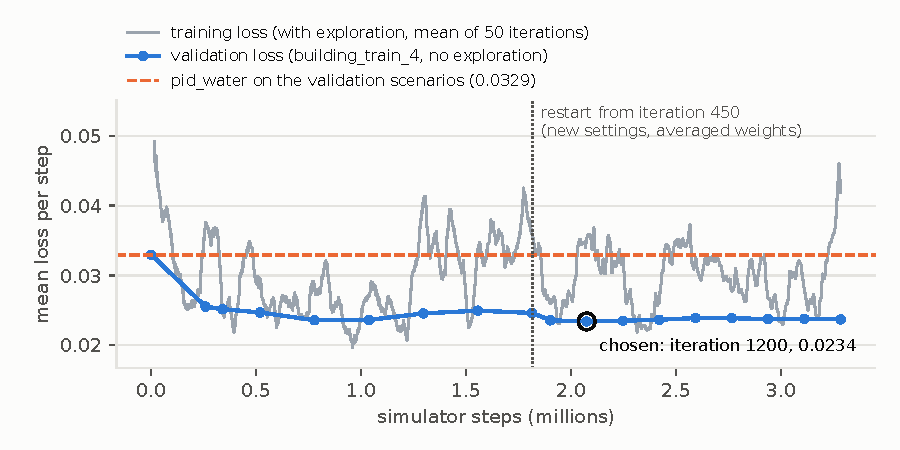
\includegraphics[width=0.86\linewidth]{../docs/fig/fig_trained.pdf}
\caption{Training of the residual controller: loss on the validation building (five scenarios, 2880 steps, no
exploration noise; corrected simulator) and the training loss (with exploration noise, mean of 50 iterations), against
simulator steps. Dashed: pid\_water on the validation scenarios.}
\label{fig:trained}
\end{figure}

\begin{table}[!htb]\centering
\caption{The trained controller on the twelve full-size buildings of rounds 6 and 7 (first 2880 steps each, shipped
simulator; the buildings of Table~\ref{tab:what}), tested once after training. Loss: mean loss per step; Comfort: mean
comfort term per step; ratio of mean losses with a 95\,\% bootstrap interval over scenarios.}\label{tab:trained}
\small
% Written by sb/run_trained.py --read from results/rl_test (do not edit by hand).
\begin{tabular}{llcccc}\toprule
Policy & Training & Loss & Comfort & Loss / pid\_water & Below pid\_water\\\midrule
pid\_water & none (official baseline) & 0.07982 & 0.06341 & 1 & --\\
trained residual & 38\,h, 3.3\,M steps & 0.07141 & 0.06016 & 0.89 (0.83--0.95) & 11 of 12\\
v16 & none (learns online) & 0.01427 & 0.00048 & 0.18 (0.13--0.24) & 12 of 12\\\bottomrule
\end{tabular}

\end{table}

% Reading rules of docs/TRAINED_BASELINE.md, fixed before training.
The rules fixed before training define a real improvement on pid\_water: at most 0.95 times its loss, and a lower
loss in at least 9 of 12 scenarios. The trained policy reached 0.89 times (95\,\% interval 0.83--0.95) and was lower in
11 of 12, so it is one. v16 beats it with this budget: v16 is lower in 12 of 12, and the trained policy's loss is 5.0
times v16's (interval 3.5--7.3). The trained policy's gain over pid\_water is energy. The energy and carbon part of its
loss is 0.69 times pid\_water's (0.82 times v16's), but its comfort term stays at 0.95 times pid\_water's, while v16's
is under 1\,\% of it (Table~\ref{tab:trained}). On the validation building, of the shipped size, it had reached 0.71 times
pid\_water's loss. Before the test we expected 0.6--1.0 times pid\_water's loss and a factor of 3--5 to v16 (our
opinion, written in the plan). Both drew on the same six shipped buildings: v16's design during development, the
trained policy for training and validation. One architecture, one budget and one seed say little about what trained
control can reach.

% Kaggle public leaderboard, one submission of the same weights (notebook submission/lb/trained_residual.ipynb,
% checked to give the same actions as the two-file policy); score read 11 Nov, 20:52 UTC.
On the public leaderboard, the same weights scored 0.03911: 0.61 times the official pid\_water
baseline (0.06404) and 3.8 times v16 (0.01031), both submitted unchanged.


\section{Timestamps of the plans}\label{app:stamps}
% docs/preregistration*/ (frozen plans, manifests and their .ots proofs; proofs upgraded and verified 30 Oct 2026,
% about 16:00 by `date`, with SocketZ/opengrid/ots.py against block headers from blockstream.info). Results first
% recorded: RESULTS_HELDOUT.md (17 Oct 13:45 UTC+2), first commits of RESULTS_ROUND2-4.md (17 Oct 15:08, 18 Oct
% 07:13, 22 Oct 12:25, UTC+2), RESULTS_ROUND5.md (22 Oct 23:46 UTC+2), docs/BIGDEV.md (screen results 27 Oct),
% RESULTS_ROUND6.md (30 Oct 03:14 UTC+1).
Before each round we wrote the plan (the frozen code's hash, the scenarios, the hypotheses and their pass marks) to a
file and sent its SHA-256 hash, and nothing else, to the OpenTimestamps calendars, which commit it to a Bitcoin
transaction. Table~\ref{tab:stamps} gives, for each plan, the start of its hash and the first block that commits to
it, checked on 30 and 31 October and 9 November 2026 against block headers from a public explorer, and the commit that first put the plan in the repository, which is self-reported. A block's time is set by its
miner and can be off by up to about an hour. Each round's runs started within minutes of the plan going to the
calendars, so a block shows only that the plan existed by its time. That time is before the first result in rounds 1,
3 and 7, the first ablation, the sensor-fault test, both public ablations and the trained policy. It is 3--18 minutes
after the first few results in rounds 2, 4, 5, 6 and 8, and 80 and 25 minutes after them in the two tests of 8
November. It is before the write-up in every case but the cold start, whose block came a minute after it
(Table~\ref{tab:stamps}). That each plan came before its round's first run
rests on the calendars' receipts and on the repository's history, in which every plan is committed before its first
run started. Round 7's plan went to the calendars at 02:21 UTC, its buildings were generated at 02:22--02:23 and its
first run started at 02:24. The plans, their manifests and the proofs are in the repository (\texttt{docs/prereg*})
and are public with the code; with them anyone can repeat the check.
\begin{table}[!htb]\centering
\caption{Bitcoin timestamps of the pre-registered plans. Hash: the first 16 hexadecimal digits of the plan file's
SHA-256. Block: the first Bitcoin block that commits to it. Committed: first commit of the plan (the stamped copy, except for the first ablation). Times in UTC, October--November 2026.}\label{tab:stamps}
\footnotesize
\setlength{\tabcolsep}{3pt}
\begin{tabular}{lllllll}\toprule
Plan & Hash & Block & Block time & Committed & First result & Write-up\\\midrule
Round 1 & \texttt{fe74aa8a8a4407cb} & 971,718 & 16 Oct, 14:07 & 16 Oct, 13:51 & 16 Oct, 18:01 & 17 Oct, 11:45\\
Round 2 & \texttt{699bce06d60774b0} & 971,780 & 16 Oct, 23:17 & 16 Oct, 22:43 & 16 Oct, 23:06 & 17 Oct, 13:08\\
Round 3 & \texttt{1426c66885a163ad} & 971,934 & 18 Oct, 02:32 & 18 Oct, 02:16 & 18 Oct, 02:36 & 18 Oct, 05:13\\
Round 4 & \texttt{e26e2d7991824600} & 972,546 & 21 Oct, 23:07 & 21 Oct, 22:42 & 21 Oct, 22:57 & 22 Oct, 10:25\\
Round 5 & \texttt{e4fce3fcec9d8a62} & 972,648 & 22 Oct, 19:26 & 22 Oct, 17:04 & 22 Oct, 19:23 & 22 Oct, 21:46\\
Full-size screens$^{a}$ & \texttt{e0da4ae880a0b91e} & 973,126 & 25 Oct, 21:00 & 25 Oct, 20:43 & 27 Oct & 27 Oct\\
Round 6 & \texttt{e4d9af8c9e155e16} & 973,762 & 30 Oct, 01:45 & 30 Oct, 01:19 & 30 Oct, 01:38 & 30 Oct, 02:14\\
Round 7 & \texttt{9b423afc0b60c256} & 973,914 & 31 Oct, 02:24 & 31 Oct, 02:21 & 31 Oct, 02:33 & 31 Oct, 03:22\\
Ablation (Section~\ref{sec:what}) & \texttt{5da4428804edc067} & 973,939 & 31 Oct, 06:31 & 31 Oct, 06:04 & 31 Oct, 06:35 & 31 Oct, 11:00\\
Round 8 & \texttt{e782910449f3d4ce} & 973,986 & 31 Oct, 15:00 & 31 Oct, 14:33 & 31 Oct, 14:42 & 31 Oct, 15:21\\
Sensor faults (App.~\ref{app:faults}) & \texttt{8d275c9827336c50} & 974,543 & 4 Nov, 15:50 & 4 Nov, 15:26 & 4 Nov, 16:33 & 6 Nov, 00:00\\
More ablations (App.~\ref{app:abl}) & \texttt{c7903b7ae0fff60e} & 975,091 & 8 Nov, 19:36 & 8 Nov, 18:05 & 8 Nov, 18:16 & 8 Nov, 22:37\\
Cold start (App.~\ref{app:abl}) & \texttt{10f221da371ffccc} & 975,108 & 8 Nov, 23:06 & 8 Nov, 22:36 & 8 Nov, 22:41 & 8 Nov, 23:05\\
Public abl.\ 1 (Tab.~\ref{tab:what}) & \texttt{623e37dd961b61df} & 975,079 & 8 Nov, 16:45 & 8 Nov, 14:44 & 9 Nov, 07:32 & 9 Nov, 07:33\\
Public abl.\ 2 (Tab.~\ref{tab:what2}) & \texttt{c90ad08b2e6ca3d6} & 975,121 & 9 Nov, 02:42 & 9 Nov, 00:08 & 10 Nov, 07:31 & 10 Nov, 07:31\\
Trained policy (App.~\ref{app:trained}) & \texttt{289e165b14900a7d} & 975,121 & 9 Nov, 02:42 & 9 Nov, 02:27 & 11 Nov, 08:25 & 11 Nov, 09:36\\\bottomrule
\multicolumn{7}{l}{\footnotesize $^{a}$Section~\ref{sec:big}. Two reference runs of v14 were written on 25 Oct at 20:43 and 20:52.}
\end{tabular}
\end{table}

\clearpage
\section{Per-round figures}\label{app:figs}
Traces and per-scenario results of the individual rounds.

\begin{figure}[!htb]\centering
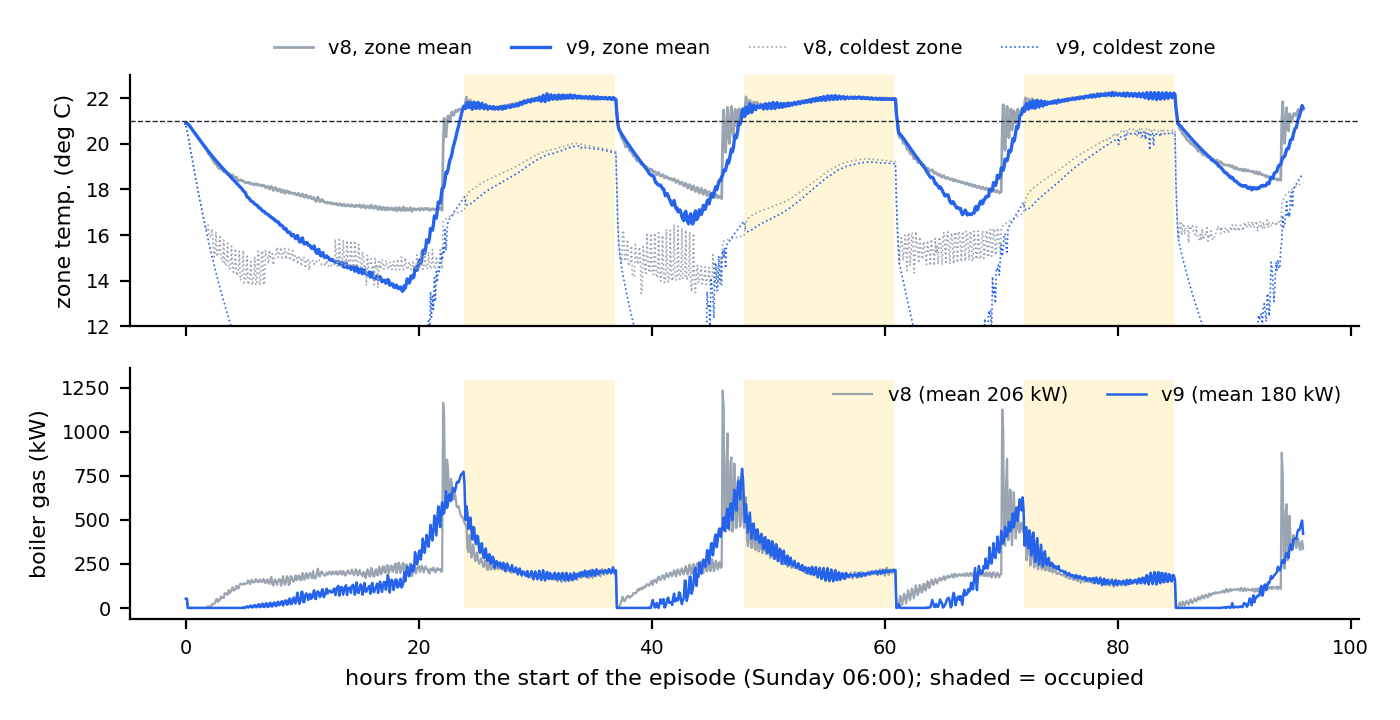
\includegraphics[width=\linewidth]{../docs/fig/fig_glide.png}
\caption{The heating-season setback (training scenario: building 2, Fairbanks, February, first four days). Top: mean
and coldest zone temperature; bottom: boiler gas. Shaded: occupied. With the setback (v9) the zones float at night and
each recovers just in time; mean gas falls from 206 to 180\,kW.}
\label{fig:glide}
\end{figure}
% sb/fig_round7.py; results/round7/{v15,chm}/*.npy and the traces results/round7_diag/*.npz (sb/run_r7_traces.py).
% Zones 33 and 47 of building 7804: occupied out-of-band K-person-steps 4318 of 4770 under v15, 1208 under v16;
% planned cooling 17682 -> 435 kW-steps; strong heat-cool switches 15-66 per work day under v15 (docs/RESULTS_ROUND7.md).
\begin{figure}[!htb]\centering
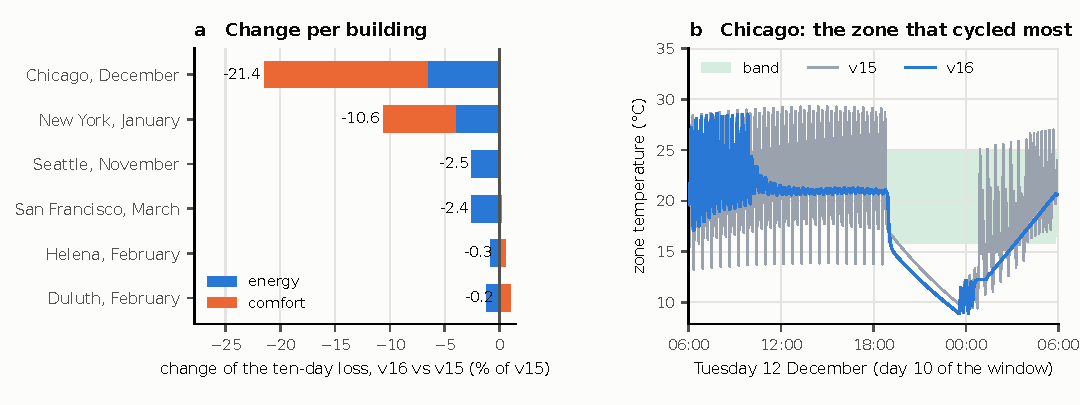
\includegraphics[width=\linewidth]{../docs/fig/fig_round7.pdf}
\caption{Round 7, v16 against v15, ten days each. (a) Change of the ten-day loss in each blind building, split into
its comfort and energy parts. (b) The zone of the Chicago building whose heat changed sign most often under v15, on
the last day: v15 alternates full heating and full cooling all day; v16 no longer cools it, still cycles on heat
during the morning recovery, and settles inside the band by 10:00.}
\label{fig:r7}
\end{figure}
% sb/fig_round6.py; results/round6h/{v14,ed1}/*.npy.
\begin{figure}[!htb]\centering
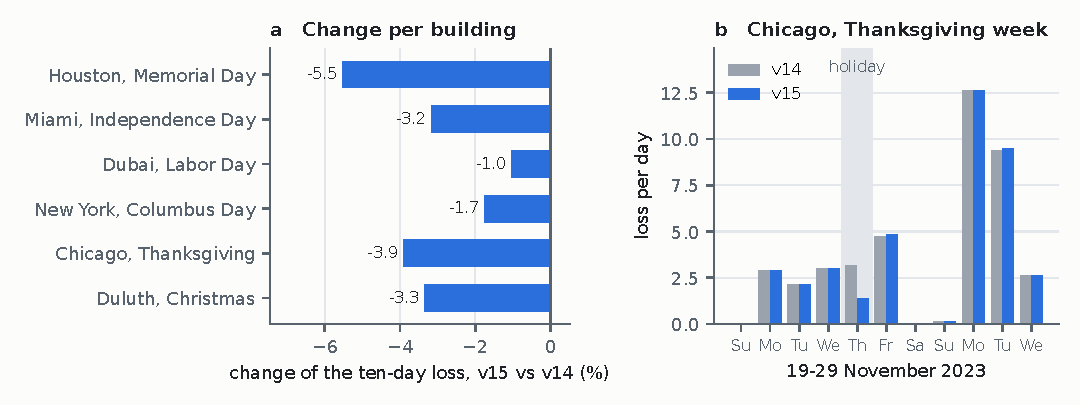
\includegraphics[width=\linewidth]{../docs/fig/fig_round6.pdf}
\caption{Round 6, v15 against v14, ten days each. (a) Change of the ten-day loss in each blind building. (b) Daily
loss in the Chicago building in Thanksgiving week: the holiday's loss falls from 3.19 to 1.40, and Friday pays back
0.11.}
\label{fig:r6}
\end{figure}
\begin{figure}[!htb]\centering
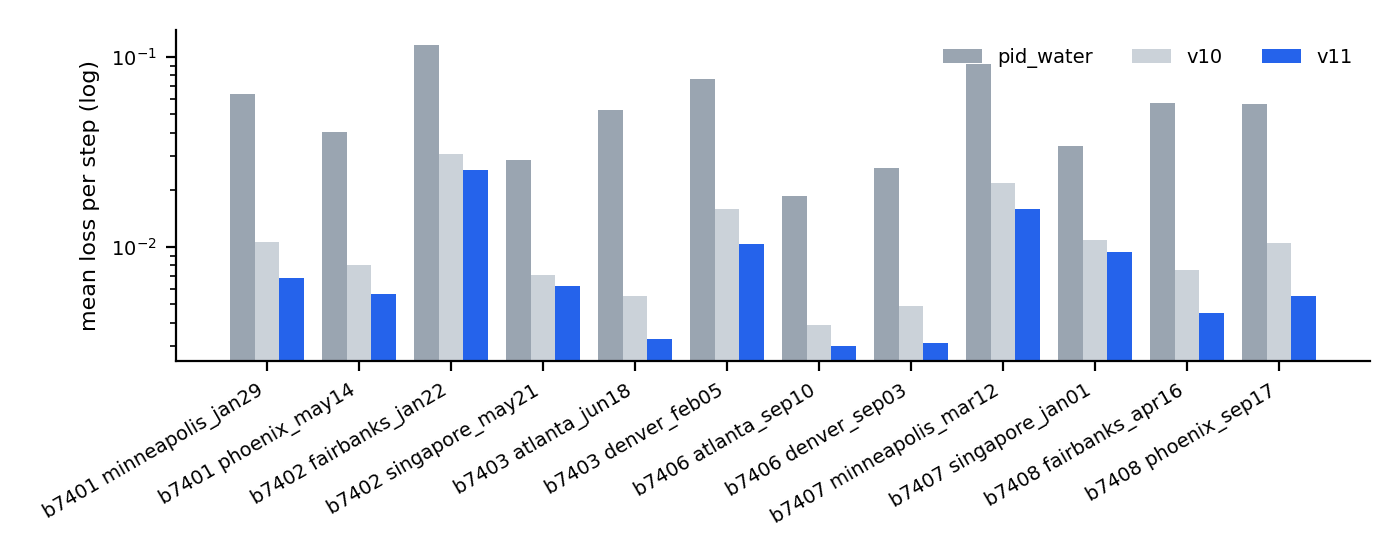
\includegraphics[width=\linewidth]{../docs/fig/fig_round5.png}
\caption{Round 5: mean loss per step in each of the 12 blind scenarios (log scale). v11 (blue) is better than v10 and
pid\_water in every scenario.}
\label{fig:r5}
\end{figure}
\begin{figure}[h]\centering
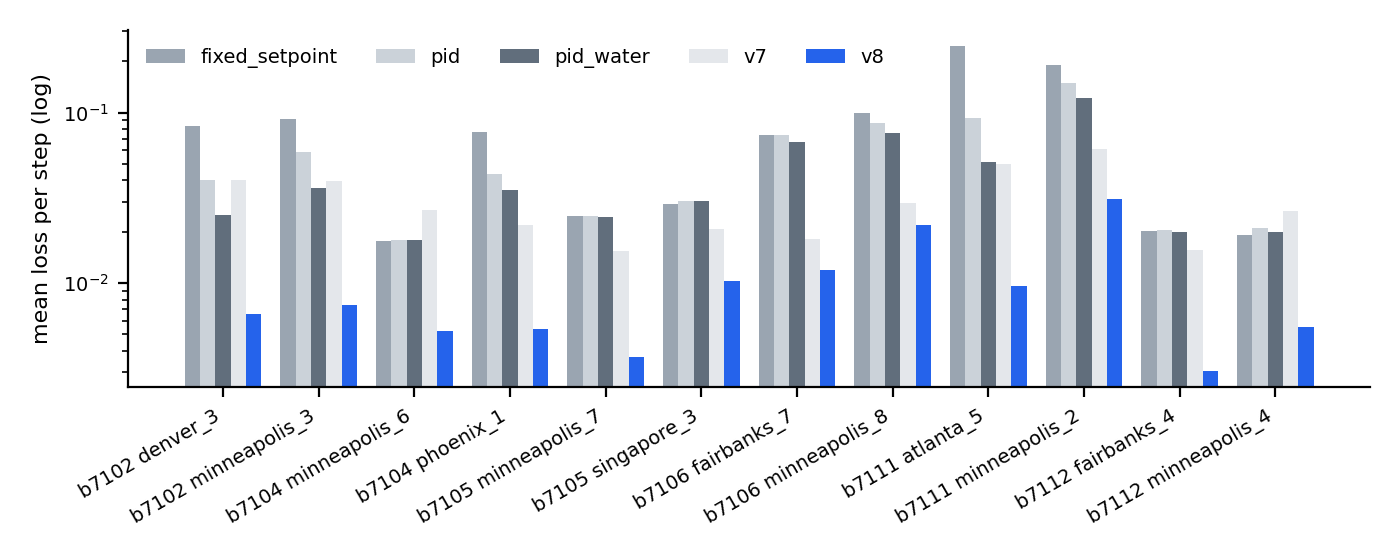
\includegraphics[width=\linewidth]{../docs/fig/fig_round2.png}
\caption{Round 2 (v8 in blue), mean loss per step per scenario (log scale).}\label{fig:r2}
\end{figure}
\begin{figure}[h]\centering
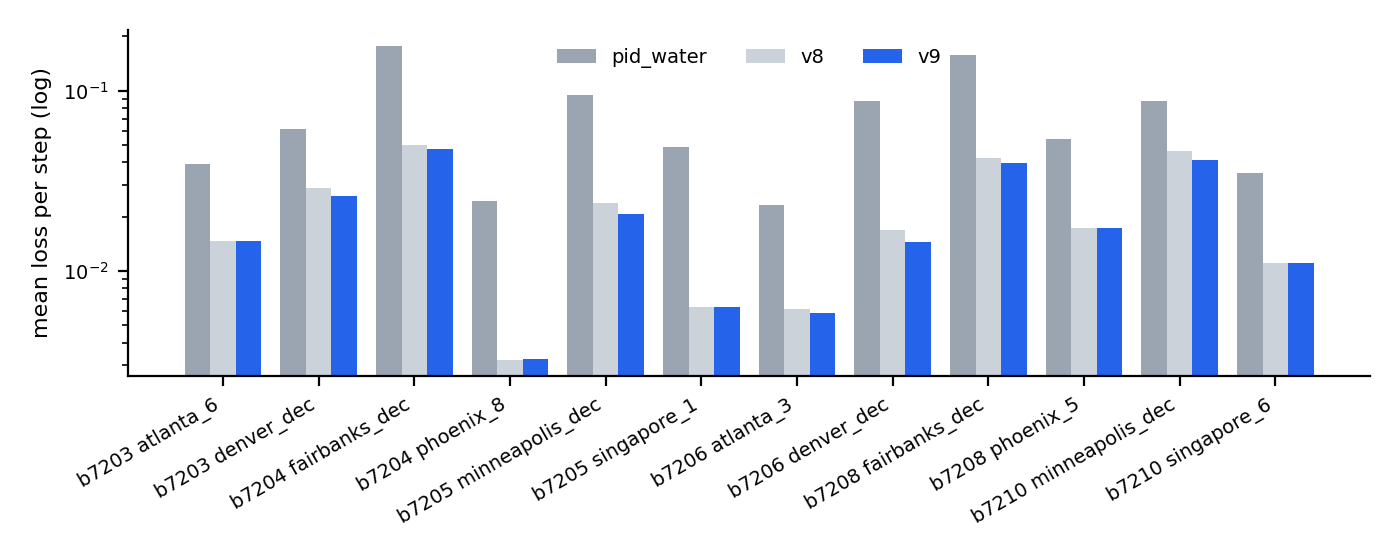
\includegraphics[width=\linewidth]{../docs/fig/fig_round3.png}
\caption{Round 3 (v9 in blue).}\label{fig:r3}
\end{figure}
\begin{figure}[h]\centering
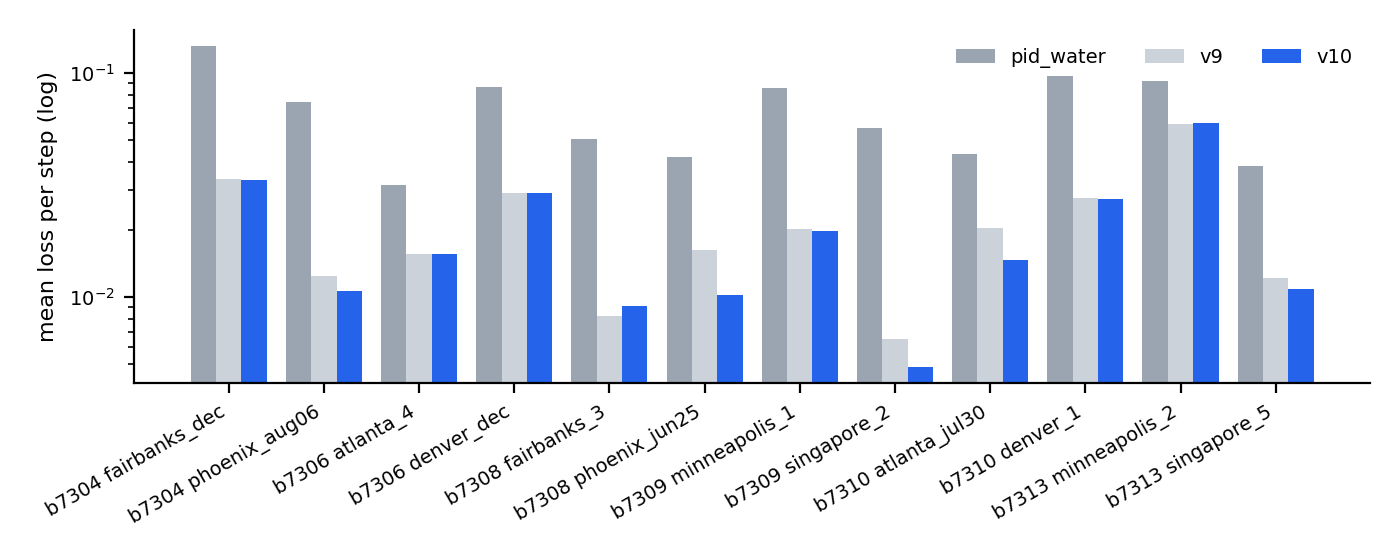
\includegraphics[width=\linewidth]{../docs/fig/fig_round4.png}
\caption{Round 4 (v10 in blue).}\label{fig:r4}
\end{figure}

\end{document}
